\documentclass[a4paper,article,14pt]{extarticle}

\usepackage{spbudiploma_tempora}
\usepackage{amsmath}
\usepackage{array}
\newcolumntype{P}[1]{>{\centering\arraybackslash}p{#1}}
\usepackage[table]{xcolor}

\usepackage{euscript}

\usepackage{longtable}
\usepackage{makecell}

\usepackage[pdftex]{graphicx}

\usepackage{amsthm, amssymb, amsmath}
\usepackage{textcomp}
\usepackage{amssymb}
\usepackage{wasysym}
\usepackage{algpseudocode}

\usepackage{scrextend}

\begin{document}

\newgeometry{left=30mm, top=20mm, right=15mm, bottom=20mm, nohead, nofoot}
\begin{titlepage}
\begin{center}

\textbf{Санкт--Петербургский}
\textbf{государственный университет}

\vspace{35mm}

\textbf{\textit{\large Шумов Дмитрий Русланович}} \\[8mm]

\textbf{\large Выпускная квалификационная работа}\\[3mm]
\textbf{\textit{\large Построение гибридной рекомендательной системы на основе коллаборативных алгоритмов и машинного обучения}}

\vspace{20mm}
Уровень образования: бакалавриат\\
Направление 01.03.02 «Прикладная математика и информатика»\\
Основная образовательная программа СВ.5005.2015
«Прикладная математика, фундаментальная информатика и программирование»\\
Профиль «Математическое обеспечение вычислительных машин,\\ комплексов и компьютерных сетей.»\\[30mm]


\begin{flushright}
{Научный руководитель:} \\
сташий преподаватель, кафедра технологии программирования,\\Стученков Александр Борисович
\end{flushright}
\begin{flushright}
{Рецензент:} \\
профессор, кафедра информационных систем,\\д.ф. - м.н.  Матросов Александр Васильевич
\end{flushright}

\vfill 

{Санкт-Петербург}
\par{2021 г.}
\end{center}
\end{titlepage}
\restoregeometry
\addtocounter{page}{1}

\tableofcontents
\pagebreak

\specialsection{Введение}

В условиях избытка информации, характерного для нашего времени, существенной является проблема её отбора.
Поэтому актуальной является разработка инструментов, позволяющих упростить эту задачу.
Рекомендательные системы призваны облегчить жизнь конечного пользователя, подстроившись под его интересы.
Они нашли широкое применение в самых различных сферах: онлайн-торговле, стриминговых сервисах, поисковых системах, рекламе.
Бизнес использует их для повышения привлекательности своих ресурсов или для увеличения продаж.
В основу рекомендательных систем легли алгоритмы коллаборативной фильтрации - простые, но допускающие большое число модификаций и комбинирование с другими алгоритмами.


\specialsection{Постановка задачи}
\textbf{Цель работы:} разработать программное обеспечение для рекомендаций пользователю фильмов.

Можно выделить следующие задачи для достижения цели работы:
\begin{itemize}
\item Исследовать популярные способы построения рекомендательных систем
\item Рассмотреть различные модификации
\item Выделить наиболее эффективный для конкретной области подход
\item Реализовать рекомендательную систему, использующую выбранный алгоритм и оценить качество её работы
\item Проанализировать полученные результаты

\end{itemize}
\pagebreak
\section{Рекомендательные системы}\label{sec:recommender_systems}
Рекомендательные системы --- компьютерные программы, используемые в попытке предсказать какому объекту пользователь отдаст своё предпочтение или какой "рейтинг"\space поставит.
Эти системы персонализируют наше взаимодействие с сетью, подсказывая что посмотреть, что купить, что послушать, с кем подружиться, что почитать и т.д. Для этого они анализируют наше взаимодействие с различными сервисами и выделяют шаблоны поведения, а также объекты, с которыми мы взаимодействуем.
Существенным для рекомендательных систем является накопление знаний об активности пользователей или свойствах объектов.
Самые базовые имплементации основываются на предположении о том, что людям понравятся вещи, похожие на те, что им уже нравятся, а также вещи, которые нравятся людям с похожим вкусом.

Рекомендательные системы можно разбить на 3 категории:
\begin{itemize}
\item На основе содержимого --- модель, которая использует множество свойств объекта для рекомендации объектов с похожими характеристиками.
\item На основе коллаборативной фильтрации --- модель, которая учитывает историю взаимодействия пользователя с сервисом (купленные товары, прослушанная музыка и т.п.), а также поведение похожих пользователей, а затем использует эту информацию для рекомендации объектов, которые могут заинтересовать пользователя.
\item Гибридные системы --- модель, сочетающая в себе два предыдущих подхода.
\end{itemize}

\subsection{Рекомендательные системы на основе \\коллаборативной фильтрации}\label{subsec:collaborative_rec_systems}
Коллаборативная фильтрация использует данные о поведении пользователей.
Данные о взаимодействии пользователей с контентом могут определяться оценками, которые пользователь поставил, и действиями, которые совершил (например, просмотрел карточку товара).
На основе этих данных система может предсказать, насколько сильно пользователю понравится объект, с которым он ещё не взаимодействовал.
Техники коллаборативной фильтрации можно разделить на 2 типа:
\begin{itemize}
\item Memory-based --- основывается на вычислении "схожести"\space пользователей или объектов их интереса
\item Model-based --- предполагает использование алгоритмов машинного обучения для предсказания пользовательского отношения к объектам
\end{itemize}
\subsubsection{Memory-based}\label{subsubsec:memory-based}
Эта техника предполагает два подхода: user-based и item-based.
User-based подход предполагает вычисление "схожести"\space между пользователями, чтобы рекомендовать конкретному человеку то, что нравится похожим на него людям.
Item-based подход предполагает вычисление "схожести"\space между объектами, чтобы рекомендовать конкретному человеку объекты, похожие на те, которыми он обычно интересуется.
Схожесть в свою очередь вычисляется, исходя из взаимосвязей пользователей и объектов.
Результатом работы является матрица предсказанных оценок, в которой построчно стоят вектора оценок для конкретного пользователя (user-based) или вектора оценок для конкретного объекта (item-based).
%Формат, впрочем, не имеет значения, так как, транспонируя матрицу, мы с лёгкостью переходим от одного представления к другому. Куда важнее, как работает сам метод.

\vspace{1em}
\textbf{Вычисление схожести}

В первых работах по коллаборативной фильтрации обычно использовалась корреляция Пирсона~\cite{resnick}:
\begin{equation}\label{eq:pearson}
    sim(u, v) = \frac
    {\sum_{i\in I_u\cap I_v}{(r_{ui} - \bar r_u)(r_{vi} - \bar r_v)}}
    {\sqrt{\sum_{i \in I_u \cap I_v}{(r_{ui} - \bar r_u)^2}}
    \sqrt{\sum_{i \in I_u \cap I_v}{(r_{vi} - \bar r_v)^2}}},
\end{equation}
где $I_u$ и $I_v$ --- множество оценок, поставленных пользователями $u$ и $v$ соответственно,
$r_{ui}$ --- оценка пользователя $u$ объекту $i$,
$\bar r_u$ --- среднее арифметическое оценок пользователя $u$.

У такого вычисления есть существенный недостаток --- оно отбрасывает объекты, оценки для которых предоставил один пользователь, но не предоставил другой.
Это может привести к тому, что два разных пользователя, одинаково оценившие несколько одних и тех же объектов, но имеющие много других оценок, будут иметь очень высокий коэффициент схожести.
Способ исправить это был предложен в~\cite{herlocker}.
Он заключается в том, чтобы домножить схожесть на $\frac{\min(\mid I_u \cap I_v\mid, n)}{n}$, тем самым уменьшая её, если у пользователей менее n общих объектов.
Частно применимая поправка, но позволяет улучшить результат.

Также для подсчёта схожести предлагалось косинусное сходство~\cite{breese}:
\begin{equation}\label{eq:cosine}
    sim(u, v) = \frac{r_u \cdot r_v}{\|r_u\| \| r_v\|{}},
\end{equation}
Однако, лучше всего себя показало центрированное косинусное сходство очень похожее на~\eqref{eq:pearson}:
\begin{equation}\label{eq:adjusted_cosine}
    sim(u, v) = \frac
    {\sum_{i \in I_u \cup I_v}{\hat{r_{ui}}\hat{r_{vi}}}}
    {\sqrt{\sum_{i \in I_u \cup I_v}{\hat{r_{ui}}^2}}
    \sqrt{\sum_{i \in I_u \cup I_v}{\hat{r_{vi}}^2}}},
\end{equation}
где
\begin{equation}
\hat{r_{ui}} =
\begin{cases}
    0, & r_{ui} = 0 \\
    r_{ui} - \bar r_{u}, & r_{ui} \neq 0
\end{cases}\label{eq:equation}
\end{equation}

Которое, ведёт себя также как и корреляция Пирсона, если пользователи оценили одинаковые объекты.
Оценки разными пользователями разных объектов всё ещё выпадают из числителя, однако увеличивают знаменатель.

\vspace{1em}
\textbf{Вычисление предсказанных оценок}

Идеи, на которых строятся способы расчёта оценок, заключаются в следующем:
\begin{itemize}
\item Чем более пользователи схожи между собой, тем большую роль играет вкус одного пользователя для другого, это можно смоделировать, взвесив оценки других пользователей.
\item Пользователи взаимодействуют с объектами по-разному: кто-то ставит более низкие оценки, кто-то оценивает только понравившиеся объекты и т. д.
Это значит, что оценки разных пользователей описываются разными распределениями, что можно учесть с помощью стандартизированной оценки~\cite{z-score}.
\end{itemize}

Таким образом, оценки вычисляются по формуле:
\begin{equation}\label{eq:z-score}
    r_{ui} = \bar r_u + \sigma_u \frac
    {\sum_{u' \in U_u}{sim(u, u')\frac{(r_{u'i} - \bar r_{u'})}{\sigma_{u'}}}}
    {\sum_{u' \in U_u}{sim(u, u')}},
\end{equation}
где $U_u$ --- множество похожих на пользователя $u$ пользователей

Итак, для составления матрицы предсказанных оценок необходимо выполнить следующие шаги:
\begin{enumerate}
\item Рассчитать коэффициенты схожести между всеми пользователями.
\item Последовательно выбирая подмножество схожих пользователей для конкретного пользователя, вычислить предсказанные оценки.
\end{enumerate}
Выше описан user-based подход, но, с точностью до перестановки пользователей и объектов, всё вышесказанное верно и для item-based подхода.

Так как в конечном итоге алгоритм составляет матрицу оценок, есть возможность совместить два этих подхода:
\begin{equation}\label{eq:memory_hybrid2}
r_{ui} = (1 - \alpha)\space UB(u, i) + \alpha\space IB(u,i)
\end{equation}
Выбирая $\alpha$, можно менять вклад каждого из подходов в конечную оценку.

\subsubsection{Model-based}
Эта техника предполагает использование алгоритмов разложения матриц и многослойных нейронных сетей.
Задача заключается в том, чтобы выявить скрытые характеристики объектов для получения недоступной ранее информации и сокращения размерности.

%\textbf{Алгоритмы разложения матриц в контексте \\рекомендательных систем}
\paragraph{Алгоритмы разложения матриц в контексте рекомендательных систем}

Как правило, пользователи взаимодействуют с небольшим количеством объектов, вследствие чего матрицы пользовательских оценок обычно сильно разряжены.
Это отрицательно сказывается на производительности рекомендательных систем.
Идея, лежащая в основе применения матричного разложения в рекомендательных системах, заключается в том, что характеристики или предпочтения пользователя могут определяться небольшим количеством скрытых факторов, которые называются эмбеддингами.
%Задача разложения матрицы может быть переформулирована как задача оптимизации с определённой функцией потерь и накладываемыми ограничениями.
%Ограничения выбираются на основе свойств нашей модели, например, матрица оценок содержит неотрицательные значения.

Суть матричного разложения представлена на рисунке~\ref{fig:mf}:
\begin{figure}[h!]
\center{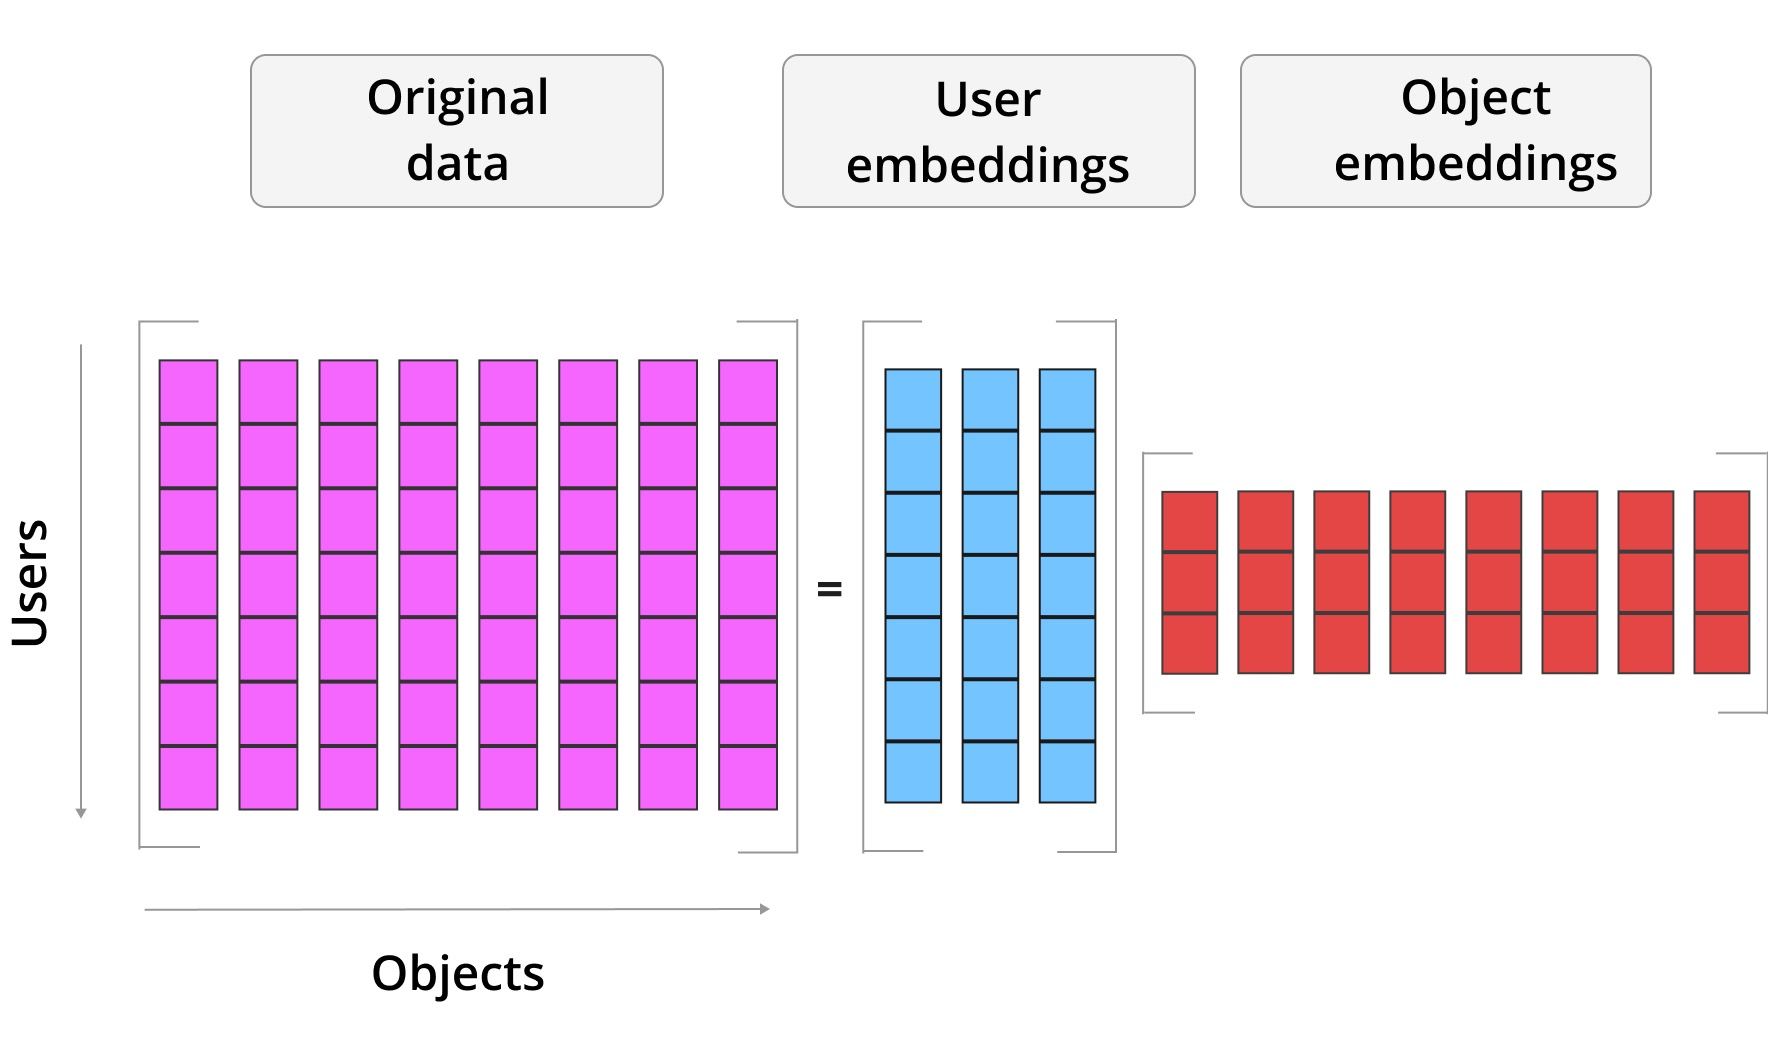
\includegraphics[scale=0.25]{images/mf_idea}}
\caption{}
\label{fig:mf}
\end{figure}

Эмбеддинги можно понимать как вектора скрытых свойств, присущих пользователям и объектам, как правило, обладающие низкой размерностью.
Матрицы, полученные в ходе разложения, являются матрицами эмбеддингов.

Задача разложения матрицы может быть переформулирована как задача оптимизации с определённой функцией потерь.
Для нахождения разложения матрицы эмбеддингов инициализируются случайными элементами, а далее, путем минимизации ошибки рассчитываются актуальные значения.
В процессе матричного разложения значения в исходной матрице аппроксимируются значениями реконструированной матрицы, разряженность которой снижается, что значит, что мы получаем значения для неизвестных (нулевых) элементов исходной матрицы.
Предсказанная оценка для пары пользователь-объект суть произведение соответствующих векторов матриц разложения.

\vspace{1em}
\textbf{Alternating Least Squares}


Зададим предсказанную оценку как произведение векторов, соответствующих пользователю и объекту:
\begin{equation}\label{eq:1}
    \hat{r_{ui}} = U_{u} \cdot V_{i}
\end{equation}
где $U_{u}, V_{i}$ --- вектора скрытых признаков пользователя и объекта соответственно.

Тогда функция потерь может быть задана следующим образом:
\begin{equation}\label{eq:2}
        L = \sum_{u, i\in S}{(r_{ui} - U_{u} \cdot V_{i}) ^ 2}
\end{equation}
где $S$ --- множество пар пользователей/объектов, с которыми производилось взаимодействие.

Для защиты от переобучения используется L2-регуляризация~\cite{l-reg}
\begin{equation}\label{eq:3}
        L = \sum_{u, i\in S}{(r_{ui} - U_{u} \cdot V_{i}) ^ 2} + \lambda_{U}\sum_{u}{\|U_{u}\| ^ 2} + \lambda_{V}\sum_{i}{\|V_{i}\| ^ 2}
\end{equation}
где $\lambda_{U}, \lambda_{V}$ --- гиперпараметры модели для регуляризации.


Метод предполагает минимизацию ошибки путём последовательного фиксирования одного набора векторов скрытых признаков и обновления другого.
Дифференцируя отдельно по признакам пользователей, отдельно по признакам объектов, получают выражения для производной:

\begin{equation}\label{eq:4}
        \frac{\partial L}{\partial U_{u}} = -2\sum_{i}{(r_{ui} - U_{u} \cdot V_{i})V_{i} + 2 \lambda_{U}U_{u}}
\end{equation}

\begin{equation}\label{eq:5}
        \frac{\partial L}{\partial V_{i}} = -2\sum_{u}{(r_{ui} - U_{u} \cdot V_{i})U_{i} + 2 \lambda_{V}V_{i}}
\end{equation}

Приравнивая производную к нулю, получают выражения для искомых векторов:
\begin{equation}\label{eq:6}
        U_{u} = r_{u}V(V^\intercal V + \lambda_{U} E)^{-1}
\end{equation}

\begin{equation}\label{eq:7}
        V_{i} = r_{i}U(U^\intercal U + \lambda_{V} E)^{-1}
\end{equation}

Выбрав размерность эмбеддингов и параметры регуляризации, итеративно рассчитывая новые значения целиком сначала для одного набора векторов, а затем для другого, вычисляют матрицы разложений.


\vspace{1em}
\textbf{Stochastic Gradient Descent}

Оценки разных пользователей описываются разными распределениями, то же верно и для объектов взаимодействия.
Чтобы учесть это, в модель добавляют поправку на центр распределения.

Тогда предсказанная оценка представляется следующим образом:
\begin{equation}\label{eq:8}
    \hat{r_{ui}} = \mu + \mu_u + \mu_i+ U_{u} \cdot V_{i}
\end{equation}
где $U_{u}, V_{i}$ --- вектора скрытых признаков пользователя и объекта соответственно,
$\mu, \mu_u, \mu_i$ --- общее среднее, среднее пользователя и среднее объекта соответственно.


Функция потерь с L2-регуляризацией:
\begin{equation}\label{eq:9}
        L = \sum_{u, i\in S}{(r_{ui} - \hat{r_{ui}})) ^ 2} + \lambda_{U}\sum_{u}{(\|U_{u}\| ^ 2 + \|\mu_{u}\| ^ 2)} + \lambda_{V}\sum_{i}{(\|V_{i}\| ^ 2 + \|\mu_{i}\| ^ 2)}
\end{equation}
где $S$ --- множество пар пользователей/объектов, с которыми производилось взаимодействие.

Минимизация производится посредством стохастического градиентного спуска.
Значения градиентов по переменным:

\begin{equation}\label{eq:10}
        \frac{\partial L}{\partial U_{u}} = -2\sum_{i}{(r_{ui} - \hat{r_{ui}})V_{i} + 2 \lambda_{U}U_{u}}
\end{equation}

\begin{equation}\label{eq:11}
        \frac{\partial L}{\partial V_{i}} = -2\sum_{u}{(r_{ui} - \hat{r_{ui}})U_{i} + 2 \lambda_{V}V_{i}}
\end{equation}

\begin{equation}\label{eq:12}
        \frac{\partial L}{\partial \mu_{u}} = -2\sum_{i}{(r_{ui} - \hat{r_{ui}}) + 2 \lambda_{U}\mu_{u}}
\end{equation}

\begin{equation}\label{eq:13}
        \frac{\partial L}{\partial \mu_{i}} = -2\sum_{u}{(r_{ui} - \hat{r_{ui}}) + 2 \lambda_{V}\mu_{i}}
\end{equation}

На каждой итерации вектора обновляются на основе градиента ошибки, который рассчитывается для одной или, если обучение ведётся батчами, нескольких пар оценок.
Таким образом уравнения для обновления векторов признаков записываются как:

\begin{equation}\label{eq:14}
        U_{u} = U_{i} + \nu ((r_{ui} - \hat{r_{ui}})V_{i} - \lambda_{U}U_{i})
\end{equation}
\begin{equation}\label{eq:15}
        V_{i} = V_{i} + \nu ((r_{ui} - \hat{r_{ui}})U_{u} - \lambda_{V}V_{i})
\end{equation}
\begin{equation}\label{eq:16}
        \mu_{u} = \mu_{u} + \nu (r_{ui} - \hat{r_{ui}} - \lambda_{U}\mu_{u})
\end{equation}
\begin{equation}\label{eq:17}
        \mu_{i} = \mu_{i} + \nu (r_{ui} - \hat{r_{ui}} - \lambda_{V}\mu_{i})
\end{equation}
где $\nu$ --- коэффициент скорости обучения.

Выбрав размерность эмбеддингов, параметры регуляризации и скорость обучения, итеративно вычисляют матрицы разложений.

\vspace{1em}
\textbf{Probabilistic Matrix Factorization}

Следующий подход был предложен в ~\cite{pmf}.
Идея строится на Байесовском выводе. Предполагается, что множество оценок нормально распределено относительно предсказанных оценок с общей дисперсией:
\begin{equation}\label{eq:ratings-distr}
        p(R|U, V, \sigma^2) = \prod_{u, i \in S}{N(r_{ui}|U_{u}V_{i}, \sigma^2)}
\end{equation}
где $S$ --- множество пар пользователей/объектов, с которыми производилось взаимодействие,
$N$ --- нормальное распределение.\\
Предполагается, что:
\begin{itemize}
\item Оценки независимы
\item Оценки нормально распределены с дисперсией $\sigma^2$
\end{itemize}
Распределения векторов признаков задаётся распределением Гаусса с центром в нуле:

\begin{equation}\label{eq:features-distr}
\begin{aligned}
        p(U|\sigma_{U}^2) = \prod_{u}{N(U_{u}|0, \sigma_{U}^2)} \\
        p(V|\sigma_{V}^2) = \prod_{i}{N(V_{i}|0, \sigma_{V}^2)}
\end{aligned}
\end{equation}
Предполагается, что:
\begin{itemize}
\item Вектора пользователей и объектов независимы между собой
\item Вектора пользователей и объектов нормально распределены с дисперсией $\sigma^2$
\end{itemize}
Задав априорные распределения, можно перейти к апостериорному выводу.
Исходя из правила Байеса:
\begin{equation}\label{eq:21}
        p(U,V|R, \sigma^2) = \frac{p(R|U, V, \sigma^2)p(U,V|\sigma^2)}{p(R|\sigma^2)} \propto p(R|U, V, \sigma^2)p(U,V|\sigma^2)
\end{equation}
Так как вектора признаков независимы, можно переписать выражение:
\begin{equation}\label{eq:aposteriori-probs}
        p(U,V|R, \sigma^2) = p(R|U, V, \sigma^2)p(U|\sigma_{U}^2)p(V|\sigma_{V}^2)
\end{equation}
С учётом \eqref{eq:ratings-distr} и \eqref{eq:features-distr}:
\begin{equation}\label{eq:aposteriori-inferred}
        p(U,V|R, \sigma^2) = \prod_{u, i \in S}{N(r_{ui}|U_{u}V_{i}, \sigma^2)} \prod_{u}{N(U_{u}|0, \sigma_{U}^2)} \prod_{i}{N(V_{i}|0, \sigma_{V}^2)}
\end{equation}
Максимизация этой функции эквивалентна максимизации логарифмированного её варианта.
\begin{equation}\label{eq:aposteriori-inferred}
        ln~p(U,V|R, \sigma^2) = - \frac{1}{2\sigma^2}\sum_{u, i \in S}{(r_{ui} - U_{u}V_{i})^2} - \frac{1}{2\sigma_{U}^2}\sum_{u}{\|U_{u}\|^2} - \frac{1}{2\sigma_{V}^2}\sum_{i}{\|V_{i}\|^2}
\end{equation}
Таким образом функция потерь представляется в знакомом виде:
\begin{equation}\label{eq:aposteriori-inferred}
        L = \frac{1}{2}(\sum_{u, i \in S}{(r_{ui} - U_{u}V_{i})^2} - \lambda_{U}\sum_{u}{\|U_{u}\|^2} - \lambda_{V}\sum_{i}{\|V_{i}\|^2})
\end{equation}
где $\lambda_{U} = \frac{\sigma^2}{\sigma_{U}^2}$,
$\lambda_{V} = \frac{\sigma^2}{\sigma_{V}^2}$.

Особенность PMF заключается в возможности пересчёта параметров регуляризации на каждой итерации, что позволяет вносить новую информацию в модель по мере обучения.
Для вычисления матриц разложения можно применить ALS или SGD подходы, рассмотренные ранее.

\pagebreak
\paragraph{Нейронные сети для рекомендаций}

Подход с использованием нейронных сетей можно рассматривать как модификацию подхода с использованием матричного разложения.
Идея для обучения нейронной сети основывается на том факте, что матрицы эмбеддингов, получаемые в ходе разложения матриц, могут быть смоделированы нейросетью.
Для этого используется один из слоёв сети, в качестве параметров которого выступают случайным образом инициализированные эмбеддинги.
Параметры этого слоя передаются на вход последующим слоям нейросети и в процессе обучения изменяются таким образом, чтобы давать корректные значения оценок для пар пользователей и объектов.
На рисунке~\ref{fig:nn_idea} приведена схема использования нейросетей для решения описанной задачи.
%В процессе обучения нейронная сеть самостоятельно выучивает эмбеддинги для пар пользователей и объектов так, чтобы эти пары давали корректные значения оценок.

\begin{figure}[h!]
\center{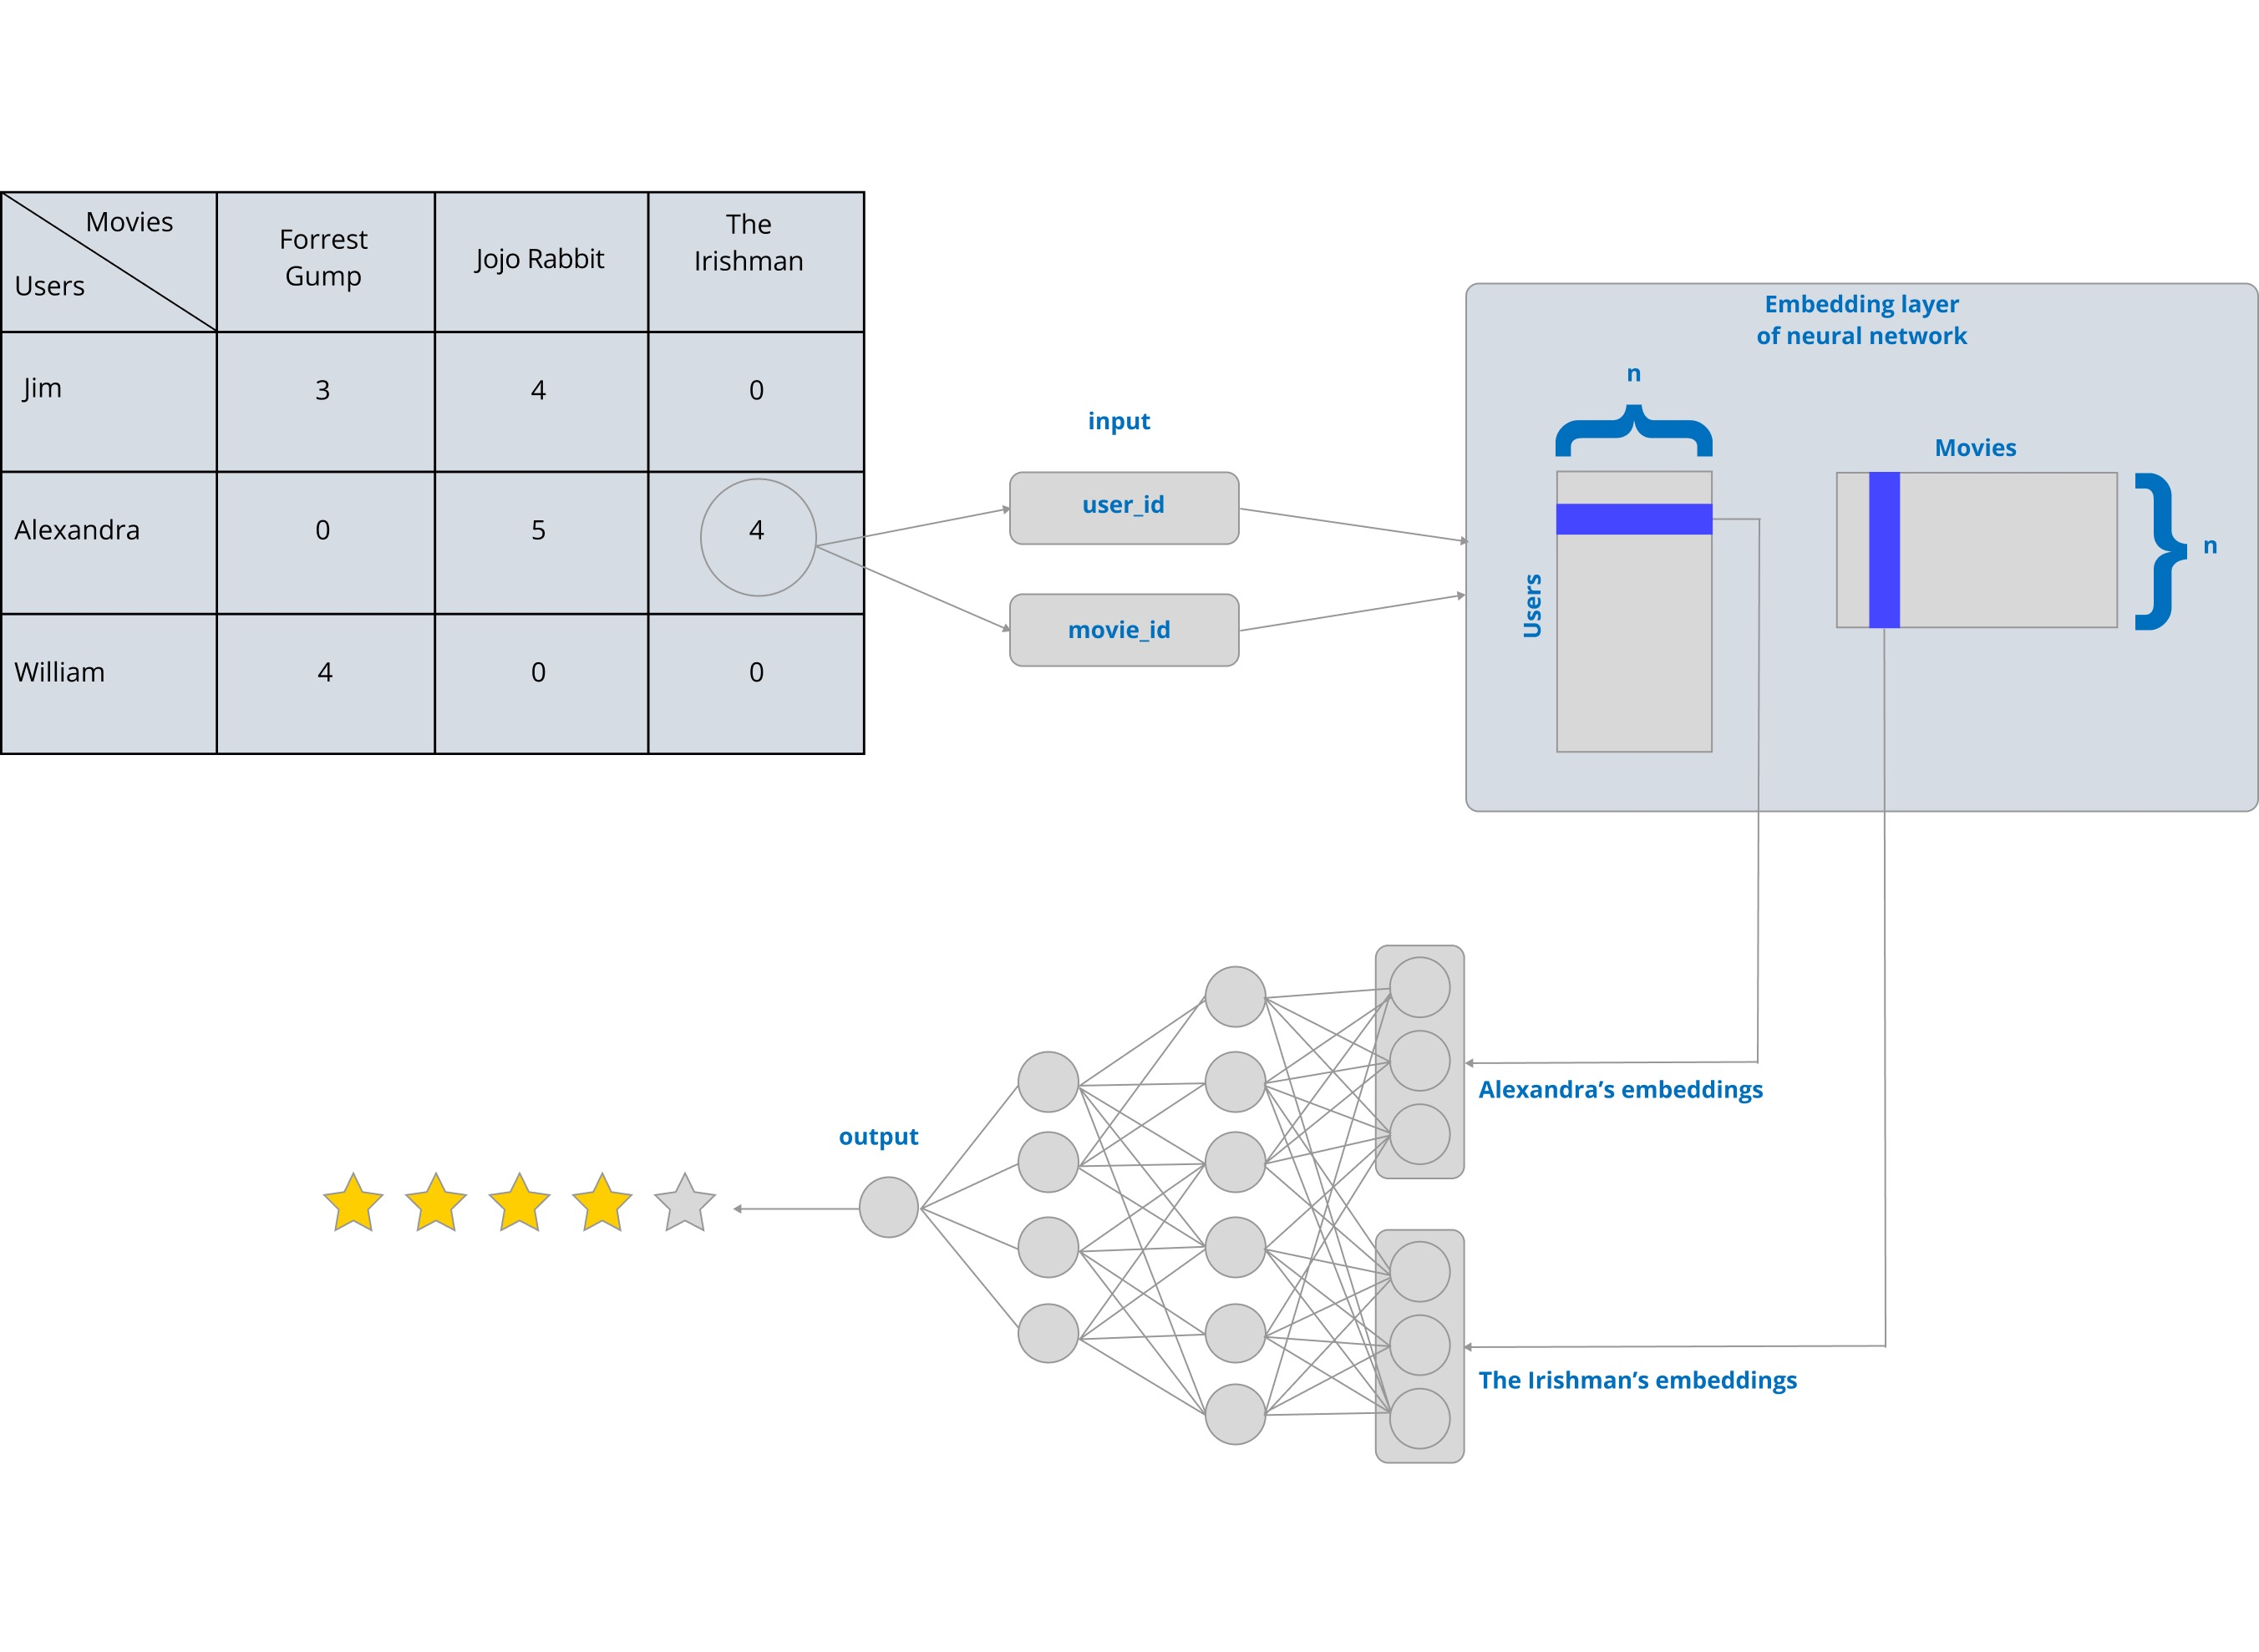
\includegraphics[scale=0.14]{images/nn_idea}}
\caption{}
\label{fig:nn_idea}
\end{figure}

\pagebreak
\subsection{Рекомендательные системы на основе содержимого}\label{subsec:content_rec_systems}
Техники коллаборативной фильтрации обладают существенным минусом --- для них актуальна проблема "холодного старта".
У новых объектов отсутствует история взаимодействий, в следствие чего модель не рекомендует их пользователям, и не происходит накопление информации.
Как правило, у объектов, с которыми взаимодествуют пользователи, можно заранее выделить некоторые признаки.
Это может быть год выхода, режиссёр, актёрский состав фильма; цена или категория товара.
На основе подобных признаков работают \textbf{content-based} алгоритмы.
\\Машинные алгоритмы не могут напрямую работать с нечисловыми признаками, такими как тэги фильма.
Чтобы получить числовое представление таких признаков, можно использовать \textbf{TF-IDF}~\cite{tfidf} (TF — term frequency, IDF — inverse document frequency).
Объекты представляются в виде документов, в которые включаются все словесные признаки.
TF-IDF мера вычисляется по следующим формулам:
\\\textbf{TF} --- отношение числа вхождений некоторого слова к общему числу слов документа.
\begin{equation}\label{eq:tf}
        tf(t, d) = \frac{n_{t}}{\sum_{k}{n_{k}}}
\end{equation}
где $n_{k}$ --- число вхождений слова $k$ в документ $d$.
\\\textbf{IDF} --- инвертированная частота, с которым слово встречается в корпусе.
\begin{equation}\label{eq:idf}
        idf(t, D) = log~\frac{\|D\|}{\|\{d_{i} \in D \| t \in d_{i}\}\|}
\end{equation}
где $D$ --- множество документов в корпусе.
\\Мера \textbf{TF-IDF}.
\begin{equation}\label{eq:tf-idf}
        tf\textnormal{-}idf(t, d, D) = tf(t, d) \times idf(t, D)
\end{equation}

Но такое представление фрагментированно и избыточно, так как каждому слову будет соответствовать отдельное измерение, и вектора, соответствующие синонимичным словам, будут ортогональны.
Чтобы сжать пространство можно использовать автоэнкодеры~\cite{autoencoders} - специальные нейросети, обученные предсказывать то же, что получили на вход.
Архитектура автоэнкодера представлена на рисунке~\ref{fig:autoencoder_simple}:

\begin{figure}[h!]
\center{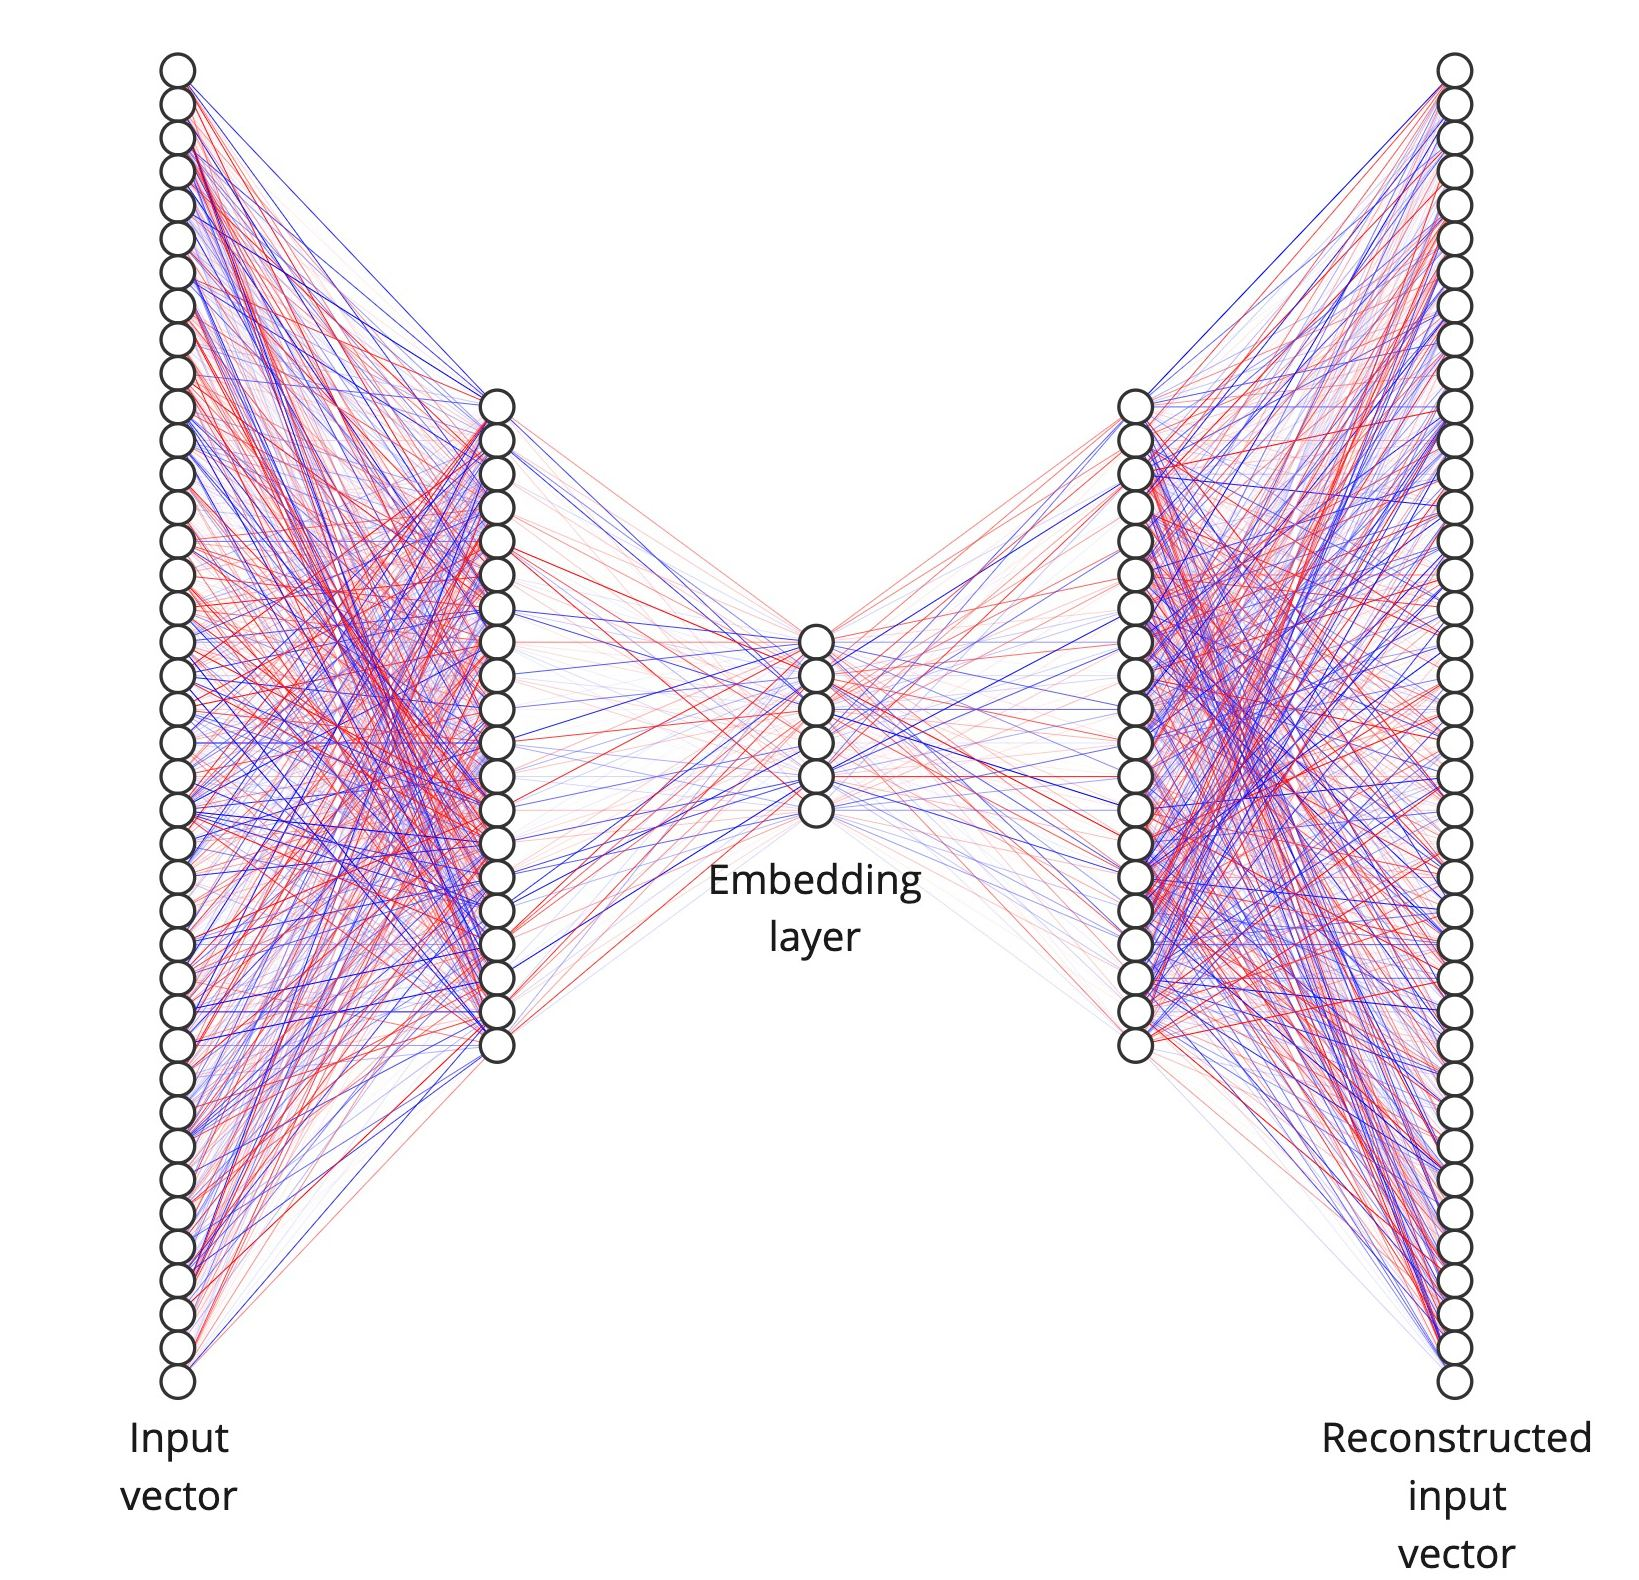
\includegraphics[scale=0.25]{images/autoencoder_simple}}
\caption{}
\label{fig:autoencoder_simple}
\end{figure}

Данная архитектура сжимает многомерное TF-IDF пространство в n-мерное.
Первая половина сети (энкодер) кодирует вектор, соответствующий объекту, а вторая половина (декодер) реконструирует оригинальные данные.
Сжатое представление в n-мерном пространстве моделируется центральным слоем сети.

Полученные таким образом векторные представления объектов дают возможность включать в рекомендации объекты, не имеющие истории взаимодействия.
Мы можем дополнительно получить вектор пользователя в пространстве, порождённым автоэнкодером, взяв взвешенную сумму векторов объектов, с которыми тот уже взаимодействовал.
\begin{equation}\label{eq:content-user-emb}
        U_{i}^{c} = \sum_{j \in S_i}{R_{ij}~I_{j}^{c}}
\end{equation}
где $S_i$ --- множество объектов, с которыми взаимодействовал пользователь $i$,
$R$ --- матрица оценок,
$U^c$, $I^c$ --- матрицы эмбеддингов пользователей и объектов.

Тогда релевантность объекта $j$ для пользователя $i$ может быть вычислена с помощью косинусного сходства:
\begin{equation}\label{eq:content-user-rel}
    \begin{aligned}
        & rel_{ij} = 0.5~\frac{U_{i}^{c} \cdot I_{j}^{c}}{\| U_{i}^{c} \| \| I_{j}^{c} \|} + 0.5, \\
        & rel_{ij} \in [0, 1]
    \end{aligned}
\end{equation}

Соответственно, предсказанная оценка:
\begin{equation}\label{eq:content-user-rating}
        \hat{R_{ij}} = r_{min} + (r_{max} - r_{min}) rel_{ij}
\end{equation}
где $r_{min}$, $r_{max}$ --- минимально и максимально возможные оценки.

Кроме того, есть возможность рекомендовать похожие между собой объекты, вычисляя похожесть через косинусное сходство.
\pagebreak

\subsection{Гибридные рекомендательные системы}\label{subsec:hybrid_rec_systems}
Гибридная модель сочетает в себе коллаборативные модели с контентными.
Гибридная рекомендательная система решает 3 задачи:
\begin{enumerate}
    \item Рекомендация пользователям релевантных объектов.
    \item Рекомендация объектов, похожих на заинтересовавший пользователя объект.
    \item Рекомендация объектов, похожих на заинтересовавший пользователя объект, с учётом предпочтений пользователя.
\end{enumerate}

\noindentГибридный подход предполагает двухэтапное ранжирование.

\noindentЗадача 1:
\begin{addmargin}[2em]{1em}% 1em left, 2em right
Коллаборативная модель решает какие $n$ объектов являются релевантными по отношению к пользовательскому запросу.
Затем контентная модель самостоятельно задаёт порядок ранжирования или вносит в него поправки, используя свои знания о релевантности объектов.
\end{addmargin}

\noindentЗадача 2:
\begin{addmargin}[2em]{1em}% 1em left, 2em right
Контентная модель задаёт порядок ранжирования по схожести с объектом интереса и отбирает $n$ самых близких.
\end{addmargin}

\noindentЗадача 3:
\begin{addmargin}[2em]{1em}% 1em left, 2em right
Контентная модель отбирает $n$ похожих объектов, а коллаборативная модель сортирует их с учётом весов, присвоенных объектам контентной моделью, или без.
\end{addmargin}

\noindentИ коллаборативная, и контентная модели обладают возможностью самостоятельно задавать релевантность объекта для пользователя, их решения можно совмещать.
Тогда ранжирование с учётом весов присвоенных обеими моделями математически выражается так:
\begin{equation}\label{eq:hybrid}
rel_{ij} = (1 - \alpha)\space M_1(i, j) + \alpha\space M_2(i, j)
\end{equation}
Выбирая $\alpha$, можно менять вклад модели в конечную оценку.


\pagebreak
\section{Эффективность рекомендаций}\label{sec:algos_efficiency}
\subsection{Метрики оценивания}\label{subsec:estimation_metrics}

\subsubsection{Регресионные метрики}
Точность рекомендательных систем обычно рассчитывается по одной из двух метрик: среднеквадратратическая ошибка (RMSE) и средняя абсолютная ошибка (MAE).
Обе этих метрики хорошо подходят для этой задачи, так как легко интерпретируются.
Однако, в некоторых случаях одной из них может отдаваться предпочтение в зависимости от данных.

\vspace{1em}
\textbf{Mean Absolute Error (MAE)}

Средняя абсолютная ошибка представляет собой сумму абсолютных разностей между прогнозами и фактическими значениями:
\begin{equation}\label{eq:mae}
MAE = \frac{1}{|R|} \sum_{u \in U , i \in I} |r_{ui} - \hat{r_{ui}}|
\end{equation}
Основная черта этой метрики состоит в том, что она не никак не реагирует на большую величину конкретных разностей, но даёт целостное представление о точности работы рекомендательной системы.

\vspace{1em}
\textbf{Root Mean Squared Error (RMSE)}

Среднеквадратическая ошибка усиливает вклад больших ошибок, будучи чувствительной к плохим предсказаниям:
\begin{equation}\label{eq:rmse}
RMSE = \sqrt{\frac{1}{|R|} \sum_{u \in U , i \in I} (r_{ui} - \hat{r_{ui}})^2}
\end{equation}
Также стоит заметить, что эта метрика по определению всегда не меньше MAE\@.

В~\cite{chai} утверждается, что MAE лучше описывает ошибки, имеющие равномерное распределение, в то время как RMSE --- ошибки, имеющие нормальное распределение.

\subsubsection{Метрики классификации}
На практике часто не стоит задача сделать все предсказания как можно ближе к действительности, но правильно выделить некоторое количество подходящих объектов.
Для этого удобно использовать F-меру и площадь под кривыми ошибок.

\vspace{1em}
\textbf{F-мера}

Обычно классы релевантных и нерелевантных объектов не равны между собой по количеству членов, поэтому на каждом из классов имеет смысл ввести свою метрику, а затем объединить их в агрегированный критерий качества.
Для этого используются точность (precision) --- доля положительно классифицированных объектов, являющихся релевантными, от всех положительно классифицированных объектов и полнота (recall) --- доля положительно классифицированных объектов, являющихся релевантными, от всех релевантных объектов.
\begin{equation}\label{eq:precision}
precision = \frac{TP}{TP + FP}
\end{equation}
\begin{equation}\label{eq:recall}
recall = \frac{TP}{TP + FN}
\end{equation}

\vspace{1em}
В таблице~\ref{tab:conf_matrix} представлена так называемая матрица ошибок (confusion matrix), демонстрирующая смысл приведённых обозначений:

\begin{table}[h]
\centering
    \begin{tabular}{|P{2cm}|P{5cm}|P{5cm}|}
    \hline
    & $y = 1$ & $y = 0$\\ 
    \hline
    $\hat{y} = 1$ & True Positive (TP) & False Positive (FP)\\ 
    \hline
   $\hat{y} = 0$ & False Negative (FN) & True Negative (TN)\\
    \hline
    \end{tabular}
    \caption{Confusion Matrix}
    \label{tab:conf_matrix}
\end{table}


Полнота и точность агрегируются в F-меру с параметром $\beta$, определяющим вклад точности в оценку:

\begin{equation}\label{eq:f-metric}
F_\beta = (1 + \beta^2) \frac{precision\cdot recall}{\beta^2\cdot precision + recall}
\end{equation}

\pagebreak
\textbf{AUC-ROC и AUC-PR}

Вещественные алгоритмы используют пороговое значение для определения принадлежности объекта к какому-либо классу, однако привязка метрики к конкретному порогу не является оптимальным решением.
Оценить работу алгоритма в общем позволяет площадь под кривой ошибок (Area Under Curve).
ROC-кривая (Receiver Operating Characteristic) строится по координатам True Positive Rate (TPR) и False Positive Rate (FPR), соответствующих определённому значению порога.
\begin{equation}\label{eq:tpr}
TPR = \frac{TP}{TP + FN},
\end{equation}
\begin{equation}\label{eq:fpr}
FPR = \frac{FP}{FP + TN},
\end{equation}
где TPR --- полнота, FPR --- доля неверно классифицированных объектов класса нерелевантных объектов.
PR-кривая (Precision Recall) аналогично строится по координатам precision и recall.
Примеры кривых приведены ниже на рисунках~\ref{fig:roc_curve_example},~\ref{fig:pr_curve_example}:
\begin{figure}[h!]
\centering
\begin{minipage}{.5\textwidth}
\centering
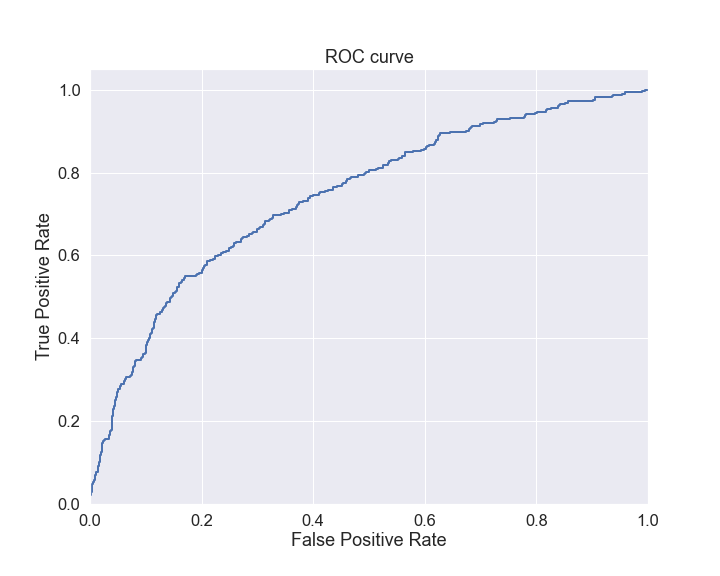
\includegraphics[width=1.1\linewidth]{images/roc_curve_example}
\caption{График ROC-кривой}
\label{fig:roc_curve_example}
\end{minipage}%
\begin{minipage}{.5\textwidth}
\centering
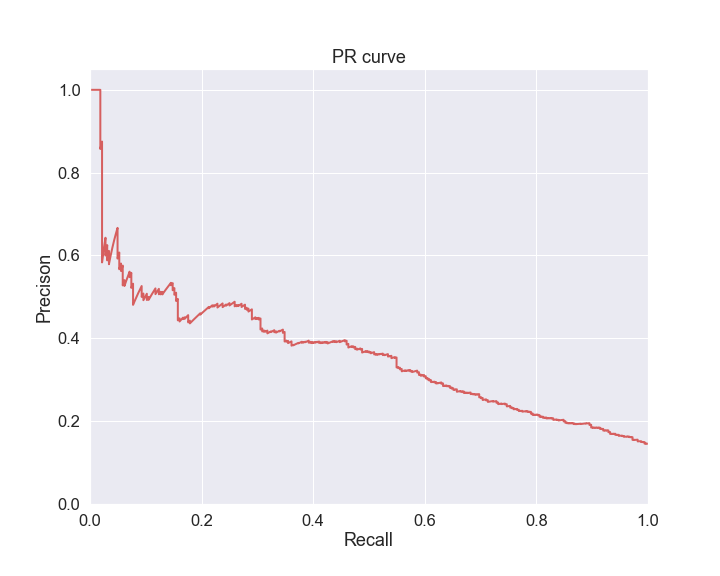
\includegraphics[width=1.1\linewidth]{images/pr_curve_example}
\caption{График PR-кривой}
\label{fig:pr_curve_example}
\end{minipage}
\end{figure}

Каждая точка на графике соответствует конкретному пороговому значению.
Чем больше площадь под кривой, тем выше качество классификации.


\subsubsection{Метрики качества ранжирования}
Зачастую может быть недостаточно предсказать оценку, которую пользователь поставит объекту, или то, окажется ли объект полезным.
В таком случае перед рекомендательной системой ставится задача ранжирования.
Задача ранжирования заключается в том, чтобы отсортировать набор элементов исходя из их релевенатности по отношению к пользователю.
В таком случае рекомендательный алгоритм помогают оценить метрики ранжирования.

Задача ранжирования может быть сформулирована следующим образом.
Рассмотрим множество пользователей $U = \{u_i\}_{i=1}^{N}$ и множество объектов $V = \{v_j\}_{j=1}^{M}$.
Результатом работы рекомендательного алгоритма является отображение $r_i: V \to \mathbb{R}$, присваивающее каждому объекту вес относительно конкретного пользователя.
Конечный набор весов задаёт для каждого пользователя перестановку $\{n_1, \dots, n_M\}$.
Для оценки качества необходимо иметь знание о степени релевантности ранжируемых объектов $\hat{r}_i$ - отображение, задающее перестановку $\{\hat{n}_1, \dots, \hat{n}_M\}$.
Истинное знание о релевантности может быть получено как за счёт имеющихся данных, так и на основе экспертной оценки.

\vspace{1em}
\textbf{Cumulative Gain(CG)}

CG представляет собой сумму истинных весов для $p$ релевантных объектов:
\begin{equation}\label{eq:cg}
CG_p = \sum_{j=1}^{p}\hat{r}_{n_j},
\end{equation}
где $\hat{r}_{n_j}$ --- истинная степень релевантности объекта на позиции $n_j$.

У метрики есть существенный недостаток - она нечувствительна к изменению порядка внутри $p$ релевантных объектов.

\vspace{1em}
\textbf{Discounted Cumulative Gain (DCG)}

DCG задаётся как~\cite{dcg}:
\begin{equation}\label{eq:dcg}
DCG_p = \sum_{j=1}^{p}\frac{\hat{r}_{n_j}}{\log_2 (j + 1)},
\end{equation}
где $\hat{r}_{n_j}$ --- истинная степень релевантности объекта на позиции $n_j$.

За счёт знаменателя метрика учитывает порядок объектов в списке.
Выбор логарифма в качестве функции дисконтирования обусловлен тем, что порядок объектов в начале списка важнее, чем в конце.
Теоретическое обоснование было дано в~\cite{dcg-log}.
Не хватает только нормализации, чтобы давать сравнимые значения для пользователей с разным количество рекомендаций.

\vspace{1em}
\textbf{Normalized Discounted Cumulative Gain (NDCG)}

Чтобы приобрести устойчивость к количеству элементов в списке - $p$, достаточно посчитать DCG для идеально отранжированного списка:
\begin{equation}\label{eq:ndcg}
NDCG_p = \frac{DCG_p}{IDCG_p},
\end{equation}
где IDCG - DCG для идеально отранжированного списка:
\begin{equation}\label{eq:idcg}
IDCG_p = \sum_{j=1}^{p}\frac{\hat{r}_{\hat{n}_j}}{\log_2 (j + 1)}
\end{equation}
Значение метрики всегда будет лежать в сегменте $[0,1]$.


\pagebreak
\subsection{Сравнение алгоритмов}\label{subsec:algos_comparison}
Каждая из моделей была обучена с полученными оптимальными гиперпараметрами.
В данном параграфе приводится оценка качества алгоритмов.
%Точность оценивается с помощью среднеквадратической ошибки и F1-меры.

Отдельного внимания заслуживают метрики классификации.
В задаче классификации определяются два класса объектов.
Вероятность принадлежности объекта $j$ к положительному классу рассчитывается следующим образом:
\begin{equation}
p_{ij} =
\begin{cases}
    0.5 + 0.5 \frac{\hat{r}_{ij} - \hat{r}_{i}^{\mean}}{\hat{r}_{i}^{\max} - \hat{r}_{i}^{\mean}}, & \hat{r}_{ij} - \hat{r}_{i}^{\mean} >= 0 \\
    0.5 - 0.5 \frac{\hat{r}_{ij} - \hat{r}_{i}^{\mean}}{\hat{r}_{i}^{\min} - \hat{r}_{i}^{\mean}}, & \hat{r}_{ij} - \hat{r}_{i}^{\mean} < 0
\end{cases}\label{eq:class_proba},
\end{equation}
где
$\hat{r}_{ij}$ --- предсказанная оценка, \\
$\hat{r}_{i}^{\mean}$, $\hat{r}_{i}^{\min}$, $\hat{r}_{i}^{\max}$ --- средняя, минимальная и максимальная предсказанные оценки пользователя.

На тестовом множестве считается, что объект относится к положительному классу, если пользователь поставил ему оценку выше своей средней.
%Для определённости в задаче классификации принято, что пользователь считает фильм плохим, если предсказанная оценка меньше его средней, и хорошим в обратном случае.

\subsubsection{Memory-based}
Схожесть будет рассчитываться с помощью центрированного косинусного сходства:

\begin{equation}
    sim(u, v) = \frac
    {\sum_{i \in I_u \cup I_v}{(r_{ui} - \bar r_u)(r_{vi} - \bar r_v)}}
    {\sqrt{\sum_{i \in I_u \cup I_v}{(r_{ui} - \bar r_u)^2}} 
    \sqrt{\sum_{i \in I_u \cup I_v}{(r_{vi} - \bar r_v)^2}}},\label{eq:equation2}
\end{equation}

Предсказанная оценка вычисляется с использованием взвешивания оценок похожих пользователей и стандартизированной оценки:
\begin{equation}
    r_{ui} = \bar r_u + \sigma_u \frac
    {\sum_{u' \in U_u}{sim(u, u')\frac{(r_{u'i} - \bar r_{u'})}{\sigma_{u'}}}}
    {\sum_{u' \in U_u}{sim(u, u')}}\label{eq:equation3}
\end{equation}

%\pagebreak
Совместим user-based и item-based подходы, определяя вклад каждого из них с помощью параметра $\alpha$.
К чистым user-based и item-based алгоритмам относятся значения $\alpha = 0$ и $\alpha = 1$ соответственно:

\begin{equation}\label{eq:memory_hybrid}
r_{ui} = (1 - \alpha)\space UB(u, i) + \alpha\space IB(u,i)
\end{equation}

Оценка качества алгоритма представлена в таблице~\ref{tab:memory_based_quality}:
\vspace{1em}
\begin{table}[h]
    \resizebox{\textwidth}{!}{%
    \begin{tabular}{ |P{4.5em}|P{2.5em}|P{2.5em}|P{2.5em}|P{2.5em}|P{2.5em}|P{2.5em}|P{2.5em}|P{2.5em}|P{2.5em}|P{2.5em}|P{2.5em}|}
    \hline
    $\alpha$ & 0 & 0.1 & 0.2 & 0.3 & 0.4 & 0.5 & 0.6 & 0.7 & 0.8 & 0.9 & 1\\
    \hline
    RMSE & 0.8847 & 0.8732 & 0.8635 & 0.8560 & 0.8504 & 0.8471 & \cellcolor{green!45}0.8458 & 0.8468 & 0.8498 & 0.8551 & 0.8624 \\
    \hline
    MAE & 0.6619 & 0.6540 & 0.6473 & 0.6420 & 0.6381 & 0.6356 & \cellcolor{green!45}0.6347 & 0.6353 & 0.6376 & 0.6415 & 0.6470 \\
    \hline
    NDCG & 0.9576 & 0.9583 & 0.9593 & 0.9601 & 0.9602 & \cellcolor{green!45}0.9607 & 0.9607 & 0.9603 & 0.9598 & 0.9592 & 0.9587 \\
    \hline
    F1 & 0.7172 & 0.7197 & 0.7224 & 0.7241 & 0.7254 & 0.7253 & 0.7257 & \cellcolor{green!45}0.7259 & 0.7239 & 0.7213 & 0.7199 \\
    \hline
    AUC-ROC & 0.7079 & 0.7126 & 0.7158 & 0.7181 & 0.7196 & 0.7207 & \cellcolor{green!45}0.7211 & 0.7202 & 0.7185 & 0.7157 & 0.7122 \\
    \hline
    AUC-PR & 0.7307 & 0.7358 & 0.7388 & 0.7406 & 0.7421 & 0.7433 & \cellcolor{green!45}0.7436 & 0.7417 & 0.7388 & 0.7353 & 0.7310 \\
    \hline
    \end{tabular}}
    \caption{Значения метрик в зависимости от $\alpha$}
    \label{tab:memory_based_quality}
\end{table}

Графики кривых при $\alpha = 0.6$ представлены на рисунках~\ref{fig:memory_based_roc},~\ref{fig:memory_based_pr}:

\begin{figure}[h!]
\centering
\begin{minipage}{.5\textwidth}
\centering
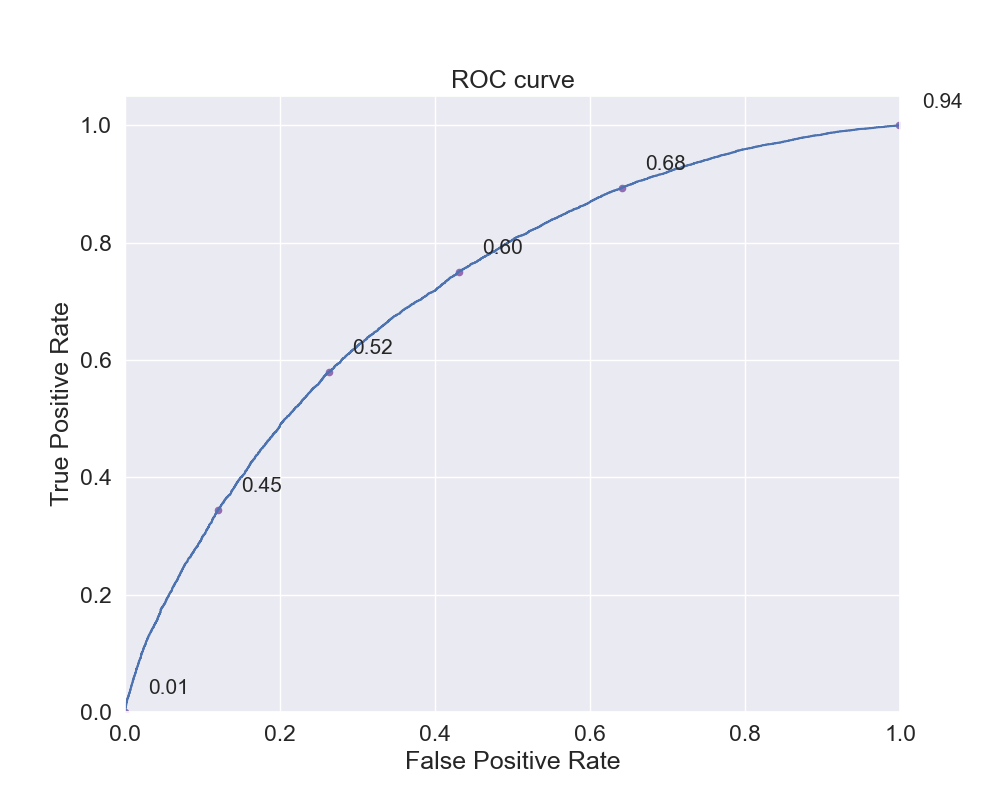
\includegraphics[width=1.1\linewidth]{images/mixed_memory_based/roc_curve}
\caption{График ROC-кривой}
\label{fig:memory_based_roc}
\end{minipage}%
\begin{minipage}{.5\textwidth}
\centering
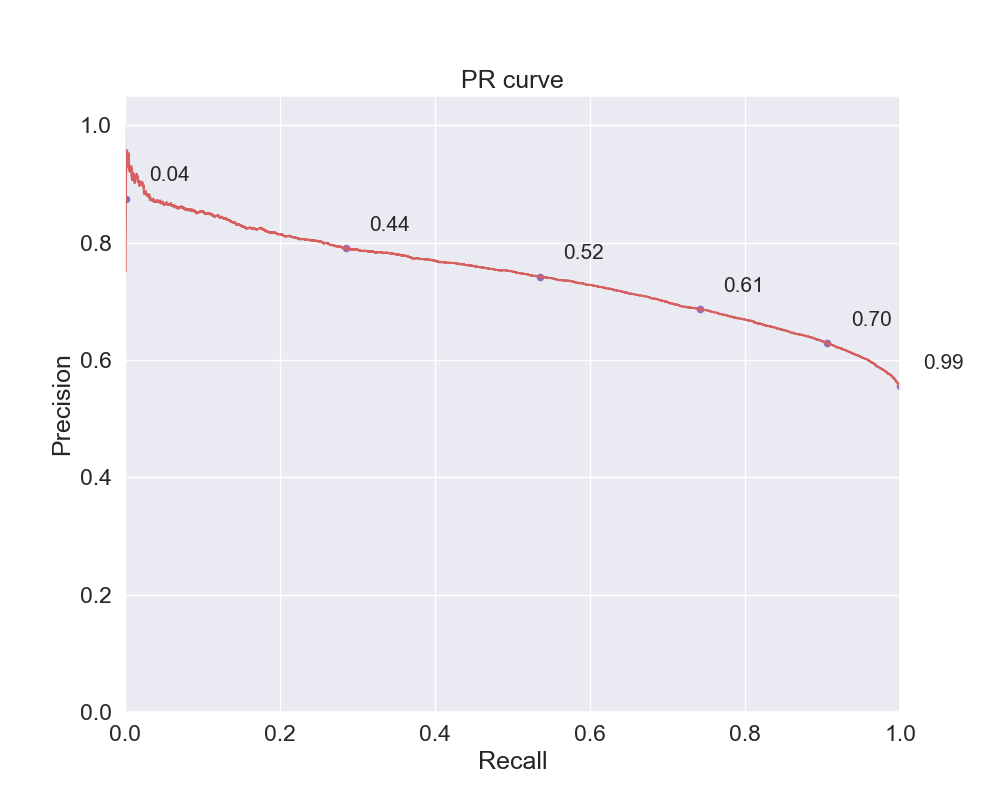
\includegraphics[width=1.1\linewidth]{images/mixed_memory_based/pr_curve}
\caption{График PR-кривой}
\label{fig:memory_based_pr}
\end{minipage}
\end{figure}

\pagebreak

\subsubsection{Model-based}
\vspace{1em}
\textbf{Alternating Least Squares}

Оценка качества представлена в таблице~\ref{tab:als_quality}:

\begin{table}[h]
    \centering{
    \begin{tabular}{ |P{4.8em}|P{4.8em}|P{4.8em}|P{4.8em}|P{4.8em}|P{4.8em}|}
    \hline
    RMSE & MAE & NDCG & F1 & AUC-ROC & AUC-PR \\
    \hline
    0.8754 & 0.6802 & 0.9609 & 0.7296 & 0.7040 & 0.7268 \\
    \hline
    \end{tabular}}
    \caption{Значения метрик для ALS}
    \label{tab:als_quality}
\end{table}

Графики ROC/PR-кривых приведены на рисунках~\ref{fig:als_roc},~\ref{fig:als_pr}:

\begin{figure}[h!]
\centering
\begin{minipage}{.5\textwidth}
\centering
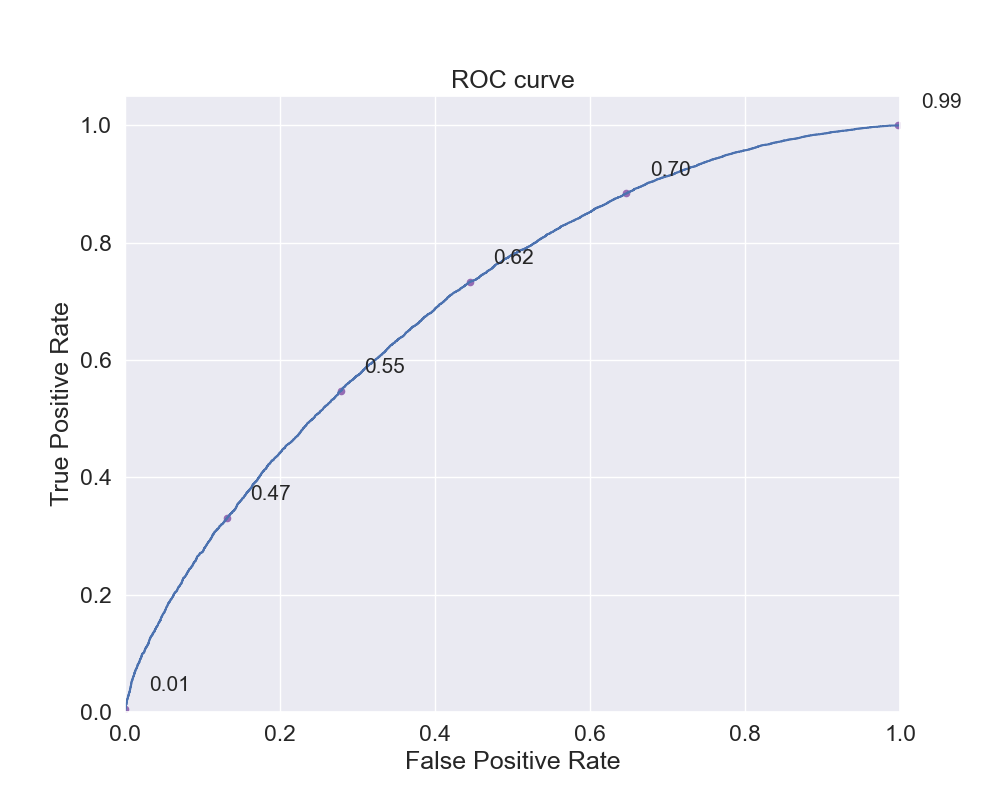
\includegraphics[width=0.9\linewidth]{images/als/roc_curve}
\caption{График ROC-кривой для ALS}
\label{fig:als_roc}
\end{minipage}%
\begin{minipage}{.5\textwidth}
\centering
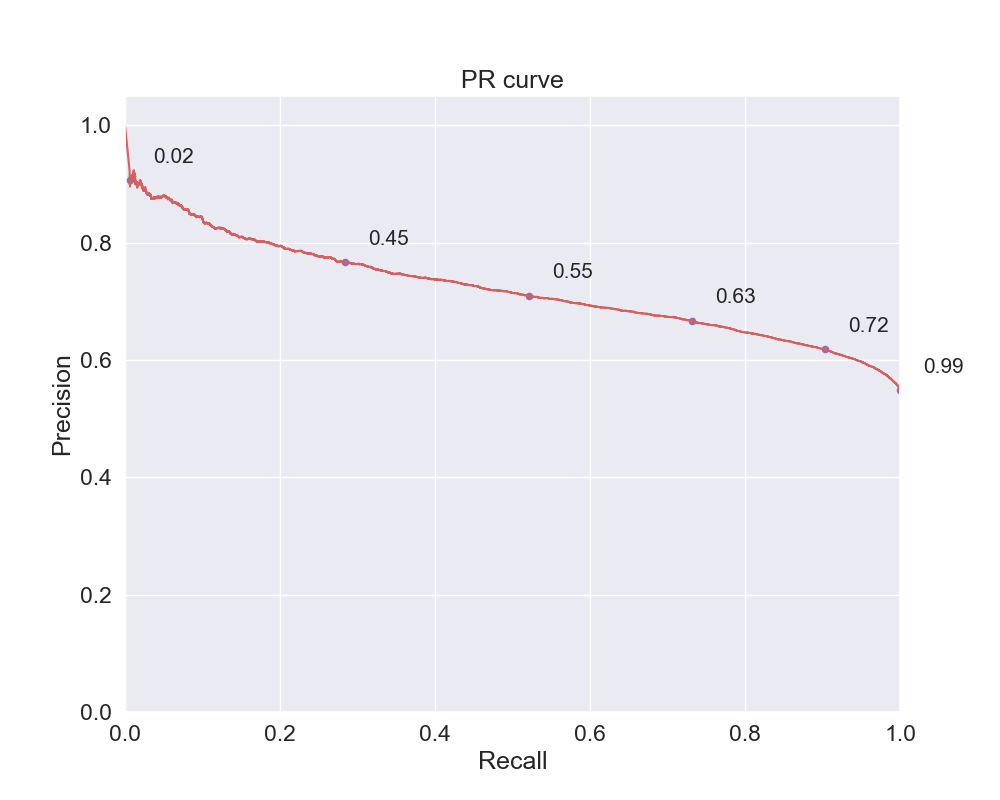
\includegraphics[width=0.9\linewidth]{images/als/pr_curve}
\caption{График PR-кривой для ALS}
\label{fig:als_pr}
\end{minipage}
\end{figure}

Значения метрик в процессе обучения представлены на рисунках~\ref{fig:als_real_losses},~\ref{fig:als_class_losses}:

\begin{figure}[h!]
\centering
\begin{minipage}{.5\textwidth}
\centering
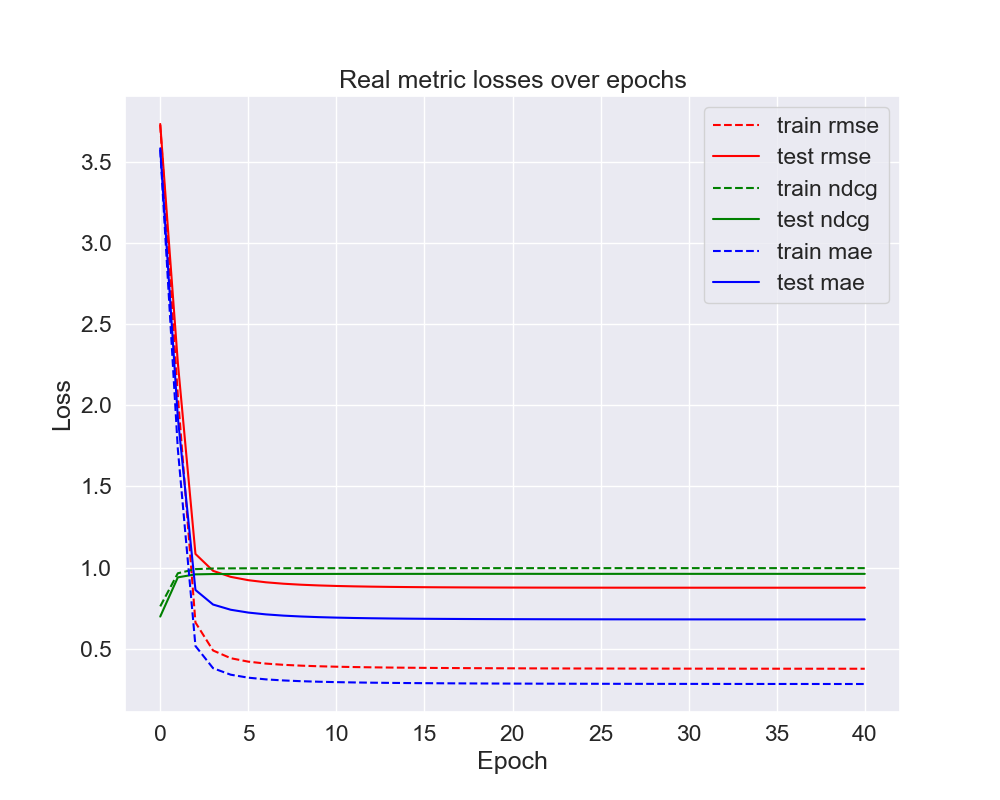
\includegraphics[width=0.9\linewidth]{images/als/real_losses}
\caption{Регрессионные метрики ALS}
\label{fig:als_real_losses}
\end{minipage}%
\begin{minipage}{.5\textwidth}
\centering
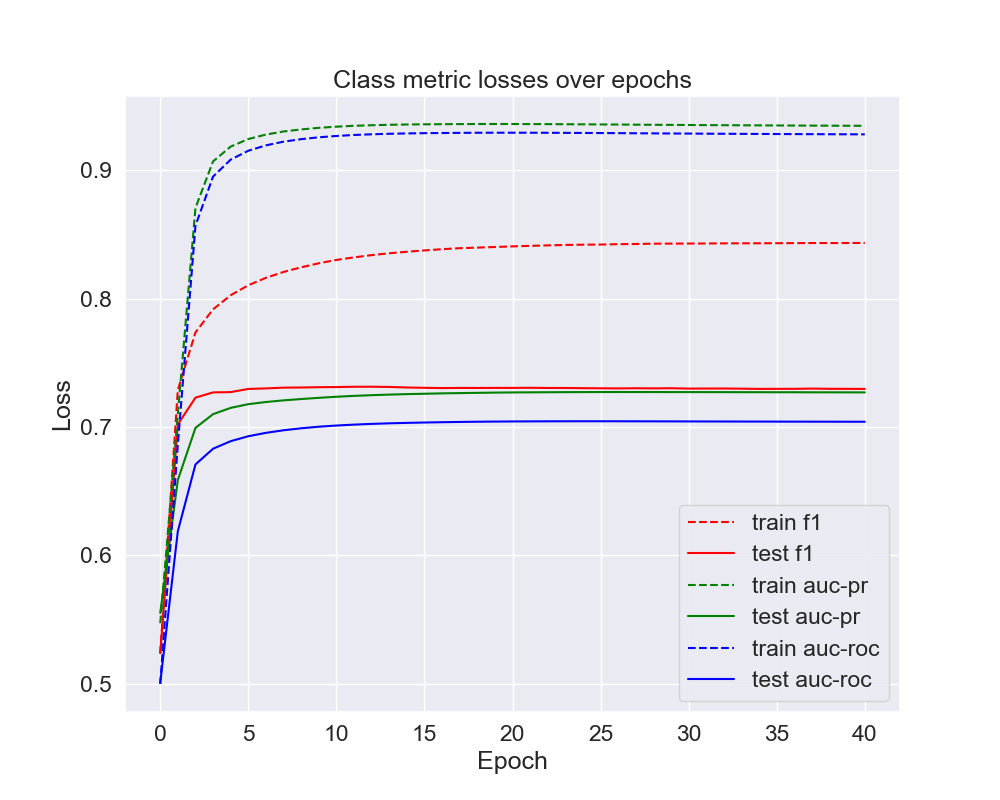
\includegraphics[width=0.9\linewidth]{images/als/class_losses}
\caption{Метрики классификации ALS}
\label{fig:als_class_losses}
\end{minipage}
\end{figure}


\pagebreak
\textbf{Stochastic Gradient Descent}

Оценка качества представлена в таблице~\ref{tab:sgd_quality}:

\begin{table}[h]
    \centering{
    \begin{tabular}{ |P{4.8em}|P{4.8em}|P{4.8em}|P{4.8em}|P{4.8em}|P{4.8em}|}
    \hline
    RMSE & MAE & NDCG & F1 & AUC-ROC & AUC-PR \\
    \hline
    0.8357 & 0.6373 & 0.9616 & 0.7287 & 0.7221 & 0.7428 \\
    \hline
    \end{tabular}}
    \caption{Значения метрик для SGD}
    \label{tab:sgd_quality}
\end{table}

Графики ROC/PR-кривых приведены на рисунках~\ref{fig:sgd_roc},~\ref{fig:sgd_pr}:

\begin{figure}[h!]
\centering
\begin{minipage}{.5\textwidth}
\centering
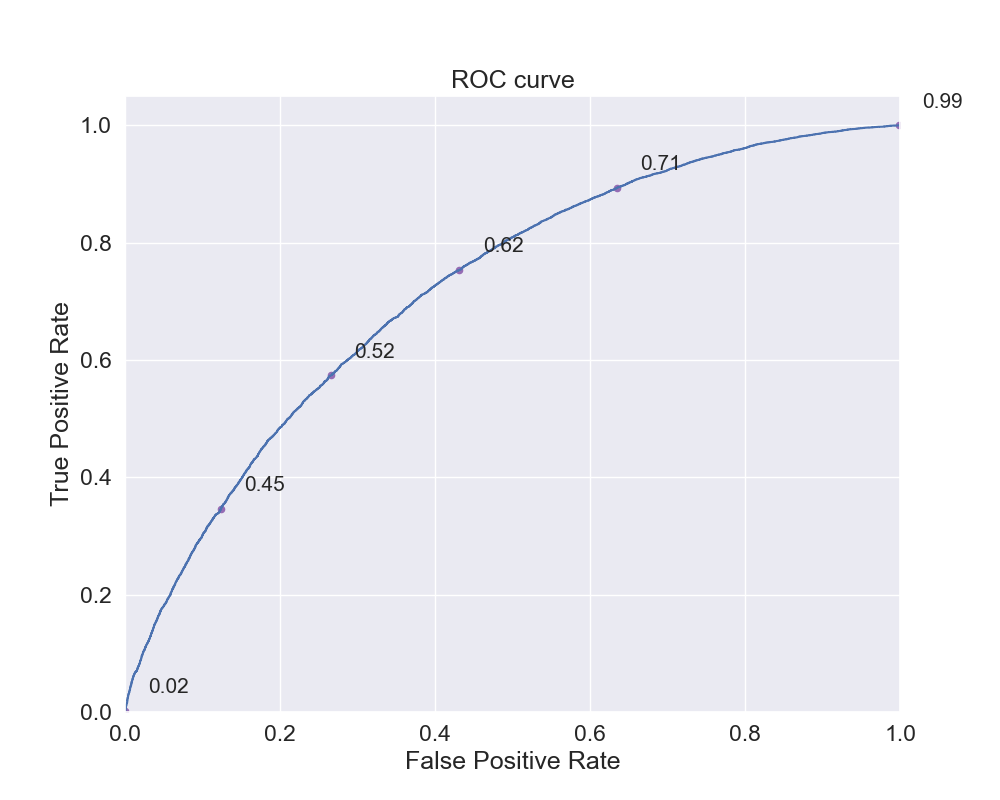
\includegraphics[width=1.0\linewidth]{images/sgd/roc_curve}
\caption{График ROC-кривой для SGD}
\label{fig:sgd_roc}
\end{minipage}%
\begin{minipage}{.5\textwidth}
\centering
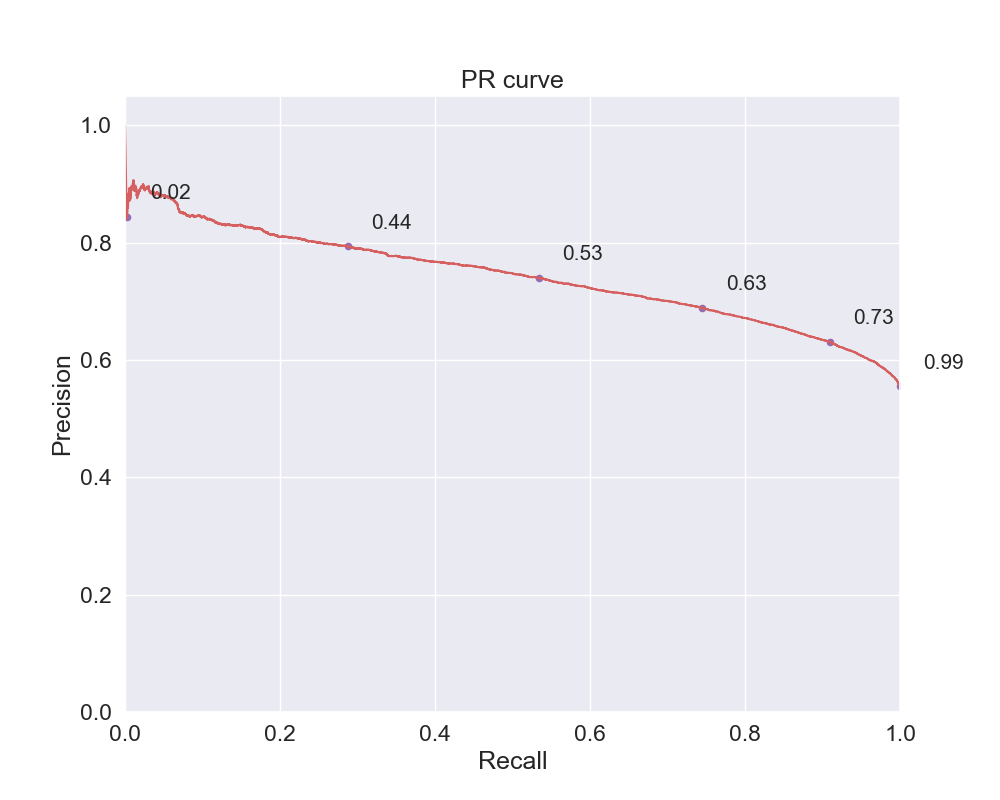
\includegraphics[width=1.0\linewidth]{images/sgd/pr_curve}
\caption{График PR-кривой для SGD}
\label{fig:sgd_pr}
\end{minipage}
\end{figure}

Значения метрик в процессе обучения представлены на рисунках~\ref{fig:sgd_real_losses},~\ref{fig:sgd_class_losses}:

\begin{figure}[h!]
\centering
\begin{minipage}{.5\textwidth}
\centering
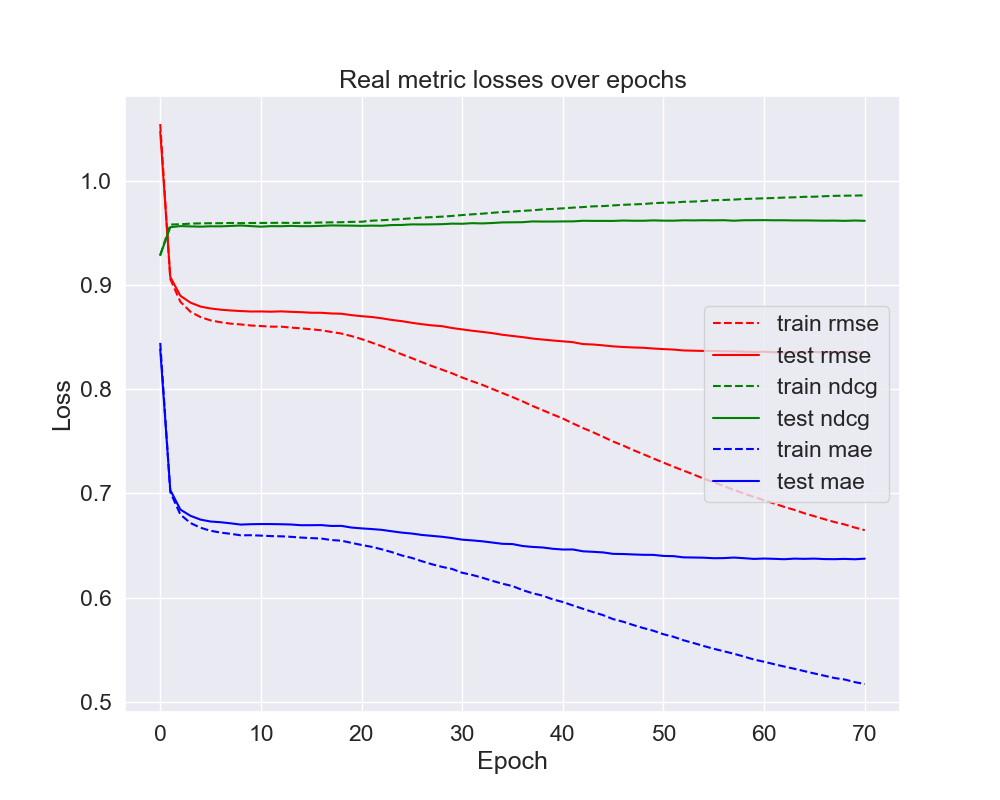
\includegraphics[width=1.0\linewidth]{images/sgd/real_losses}
\caption{Регрессионные метрики SGD}
\label{fig:sgd_real_losses}
\end{minipage}%
\begin{minipage}{.5\textwidth}
\centering
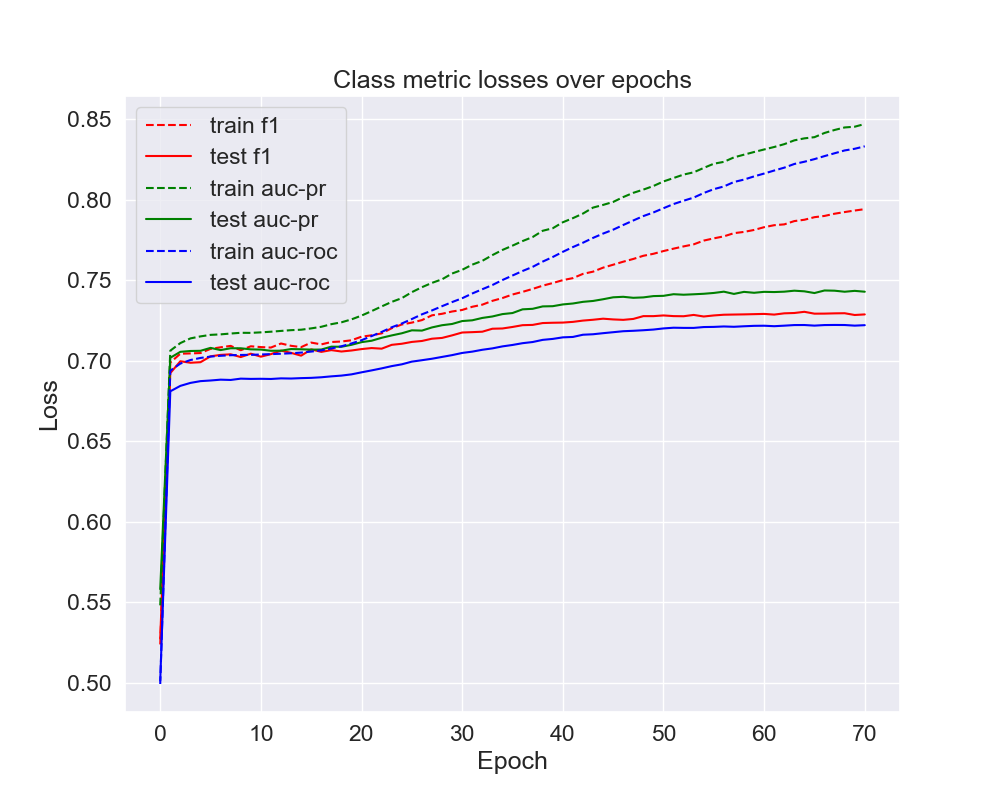
\includegraphics[width=1.0\linewidth]{images/sgd/class_losses}
\caption{Метрики классификации SGD}
\label{fig:sgd_class_losses}
\end{minipage}
\end{figure}

\pagebreak

\textbf{Probabilistic Matrix Factorization}

Оптимизация функции потерь производилась посредством SGD\@.\\
Оценка качества представлена в таблице~\ref{tab:pmf_sgd_quality}:

\begin{table}[h]
    \centering{
    \begin{tabular}{ |P{4.8em}|P{4.8em}|P{4.8em}|P{4.8em}|P{4.8em}|P{4.8em}|}
    \hline
    RMSE & MAE & NDCG & F1 & AUC-ROC & AUC-PR \\
    \hline
    0.9135 & 0.7082 & 0.9554 & 0.7127 & 0.6780 & 0.7017 \\
    \hline
    \end{tabular}}
    \caption{Значения метрик для PMF}
    \label{tab:pmf_sgd_quality}
\end{table}

Графики ROC/PR-кривых приведены на рисунках~\ref{fig:pmf_sgd_roc},~\ref{fig:pmf_sgd_pr}:

\begin{figure}[h!]
\centering
\begin{minipage}{.5\textwidth}
\centering
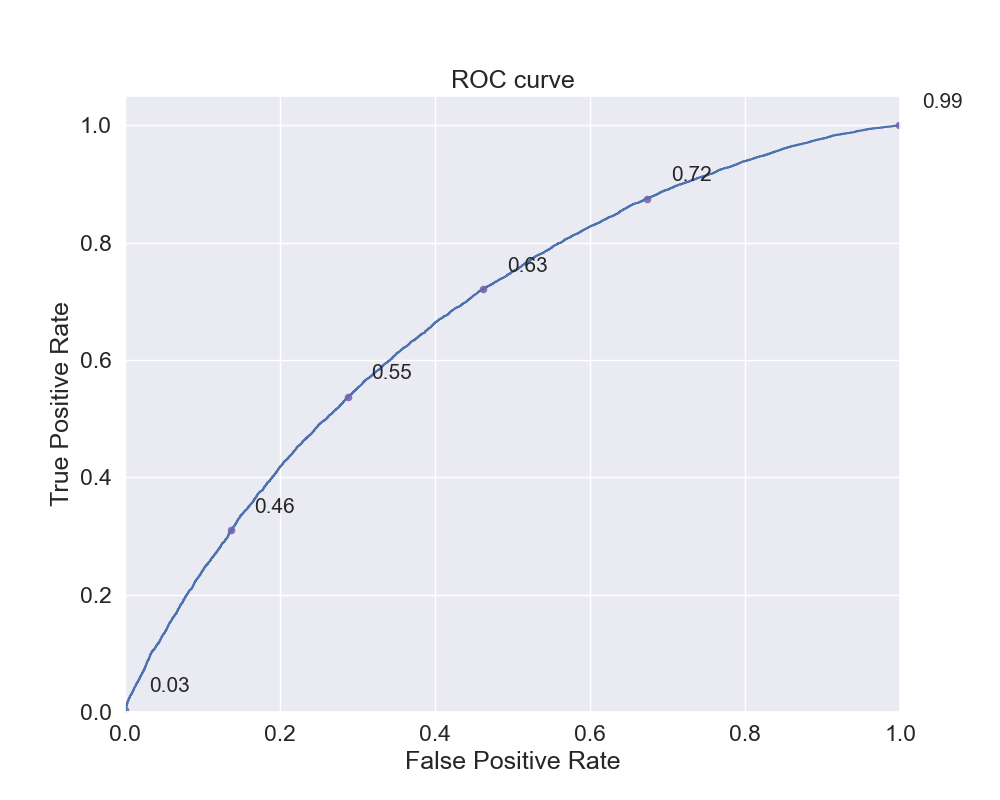
\includegraphics[width=1.0\linewidth]{images/pmf_sgd/roc_curve}
\caption{График ROC-кривой для PMF}
\label{fig:pmf_sgd_roc}
\end{minipage}%
\begin{minipage}{.5\textwidth}
\centering
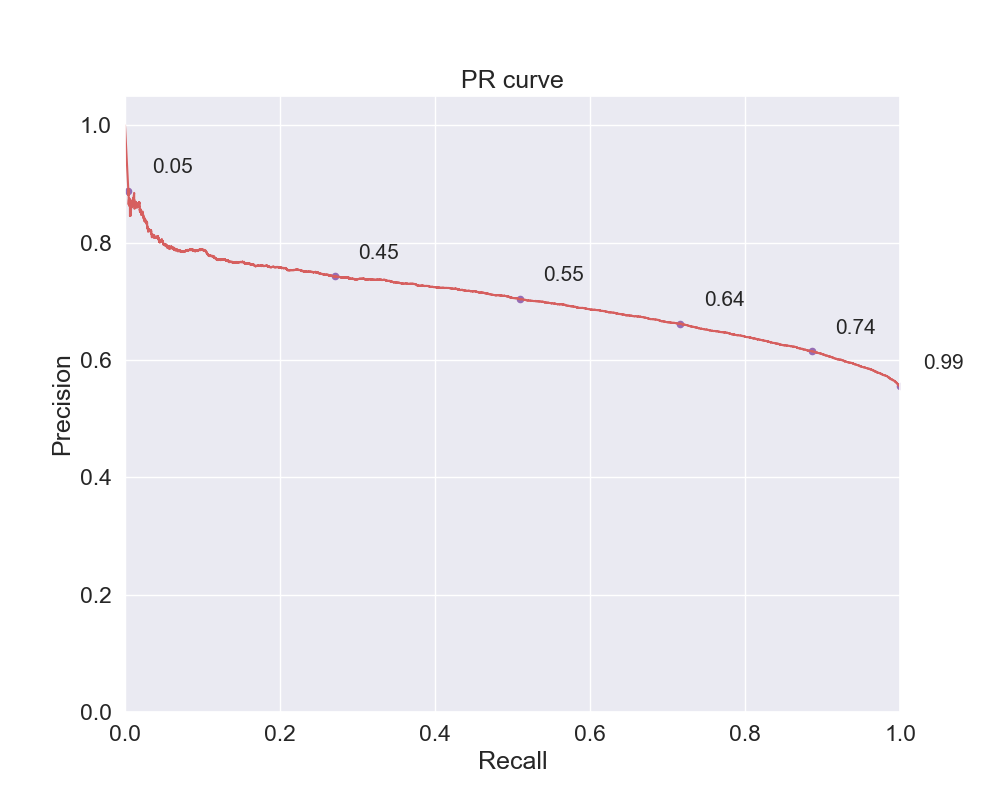
\includegraphics[width=1.0\linewidth]{images/pmf_sgd/pr_curve}
\caption{График PR-кривой для PMF}
\label{fig:pmf_sgd_pr}
\end{minipage}
\end{figure}

Значения метрик в процессе обучения представлены на рисунках~\ref{fig:pmf_sgd_real_losses},~\ref{fig:pmf_sgd_class_losses}:

\begin{figure}[h!]
\centering
\begin{minipage}{.5\textwidth}
\centering
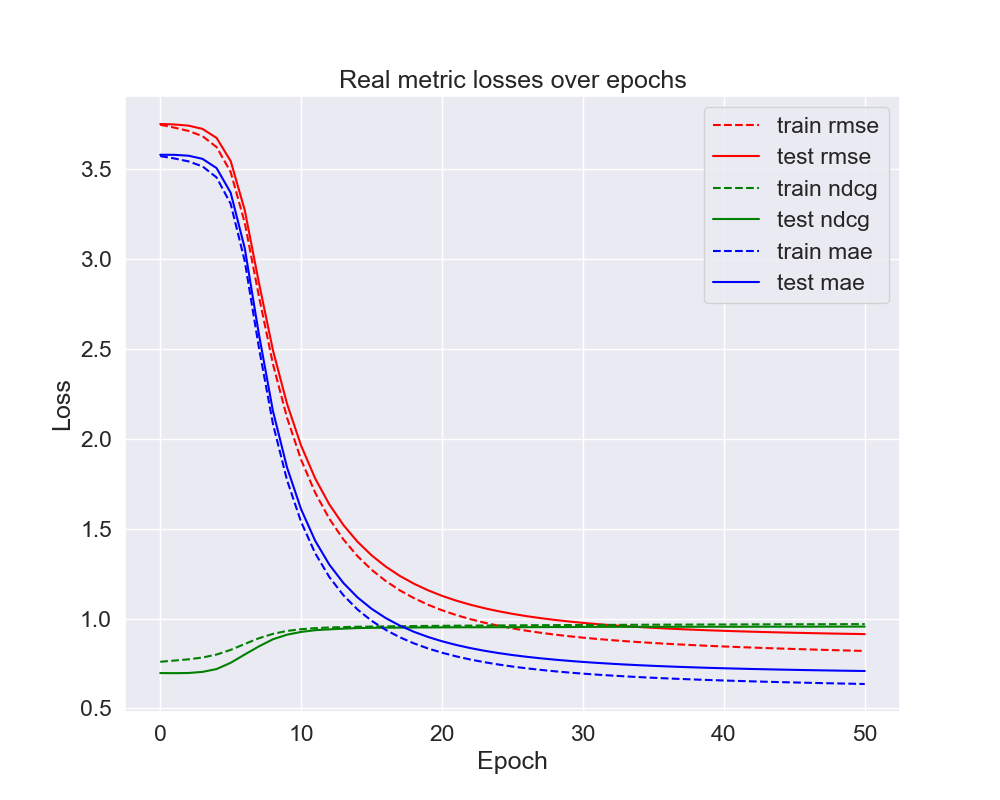
\includegraphics[width=1.0\linewidth]{images/pmf_sgd/real_losses}
\caption{Регрессионные метрики PMF}
\label{fig:pmf_sgd_real_losses}
\end{minipage}%
\begin{minipage}{.5\textwidth}
\centering
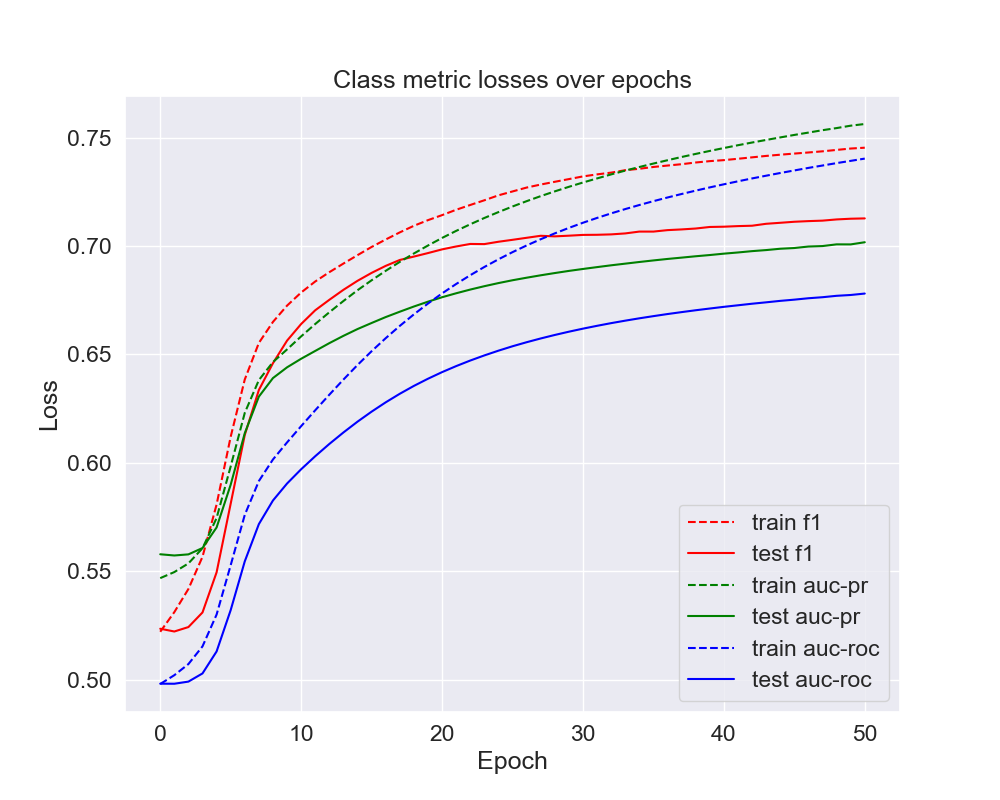
\includegraphics[width=1.0\linewidth]{images/pmf_sgd/class_losses}
\caption{Метрики классификации PMF}
\label{fig:pmf_sgd_class_losses}
\end{minipage}
\end{figure}


\pagebreak
\textbf{Neural Network}

Оценка качества представлена в таблице~\ref{tab:nn_quality}:

\begin{table}[h]
    \centering{
    \begin{tabular}{ |P{4.8em}|P{4.8em}|P{4.8em}|P{4.8em}|P{4.8em}|P{4.8em}|}
    \hline
    RMSE & MAE & NDCG & F1 & AUC-ROC & AUC-PR \\
    \hline
    0.8587 & 0.6532 & 0.9581 & 0.7130 & 0.7010 & 0.7227 \\
    \hline
    \end{tabular}}
    \caption{Значения метрик для нейросети}
    \label{tab:nn_quality}
\end{table}

Графики ROC/PR-кривых приведены на рисунках~\ref{fig:nn_roc},~\ref{fig:nn_pr}:

\begin{figure}[h!]
\centering
\begin{minipage}{.5\textwidth}
\centering
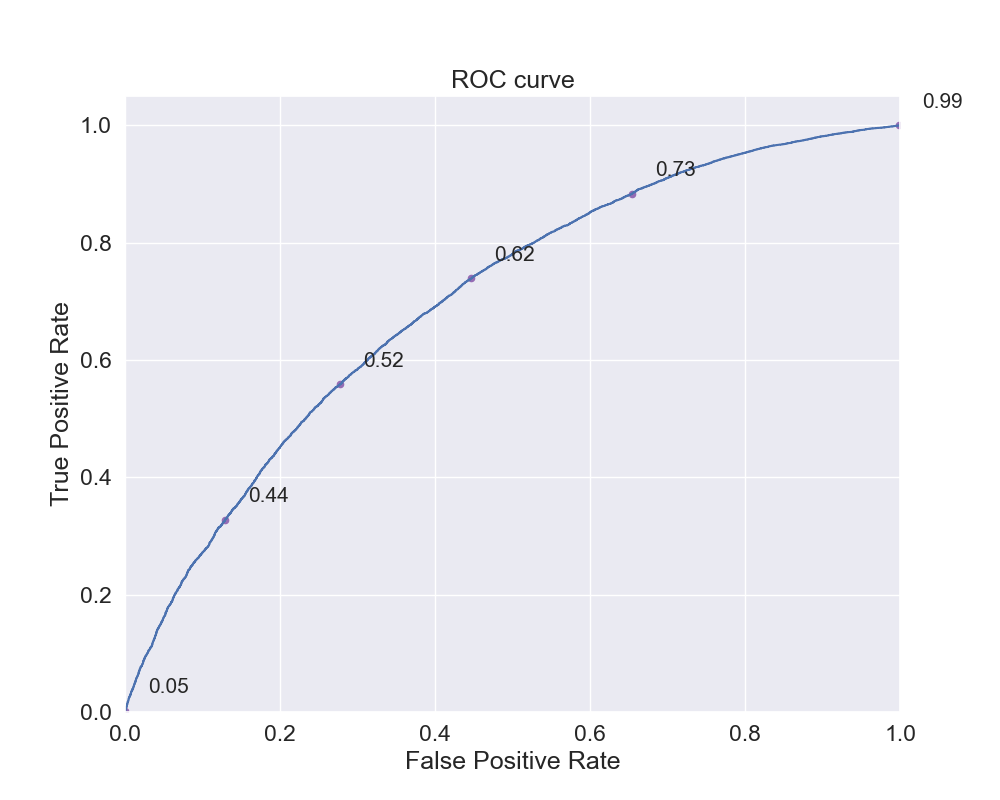
\includegraphics[width=1.0\linewidth]{images/neural_net/roc_curve}
\caption{График ROC-кривой нейросети}
\label{fig:nn_roc}
\end{minipage}%
\begin{minipage}{.5\textwidth}
\centering
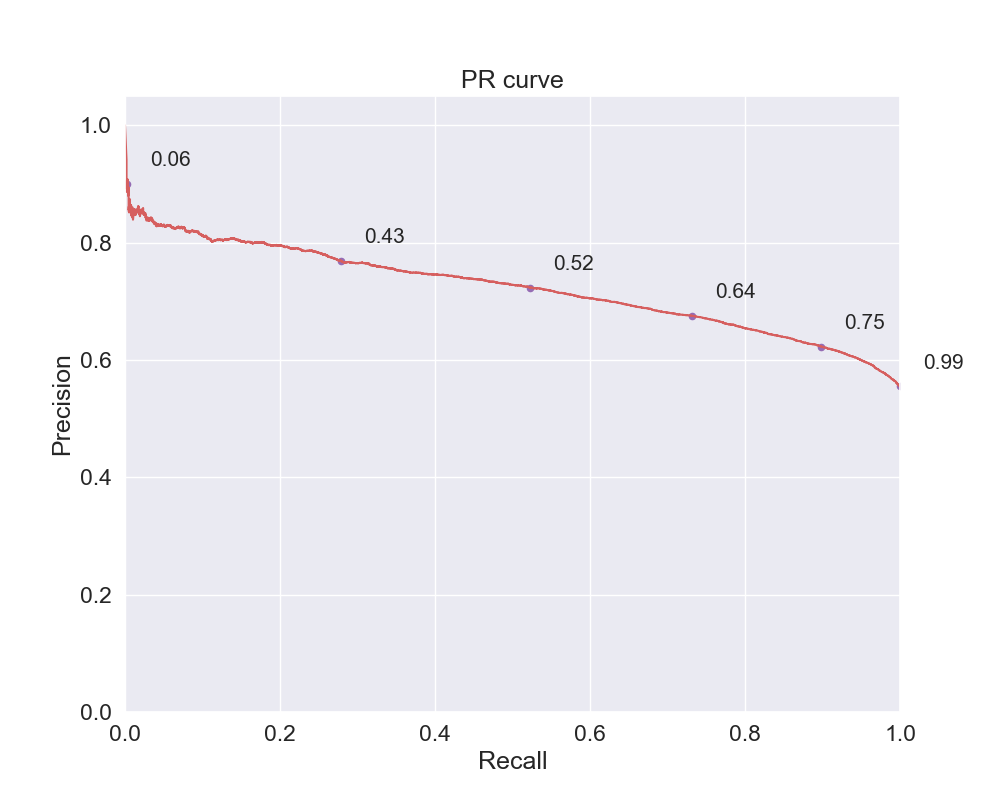
\includegraphics[width=1.0\linewidth]{images/neural_net/pr_curve}
\caption{График PR-кривой нейросети}
\label{fig:nn_pr}
\end{minipage}
\end{figure}

Значения метрик в процессе обучения представлены на рисунках~\ref{fig:nn_real_losses},~\ref{fig:nn_class_losses}:

\begin{figure}[h!]
\centering
\begin{minipage}{.5\textwidth}
\centering
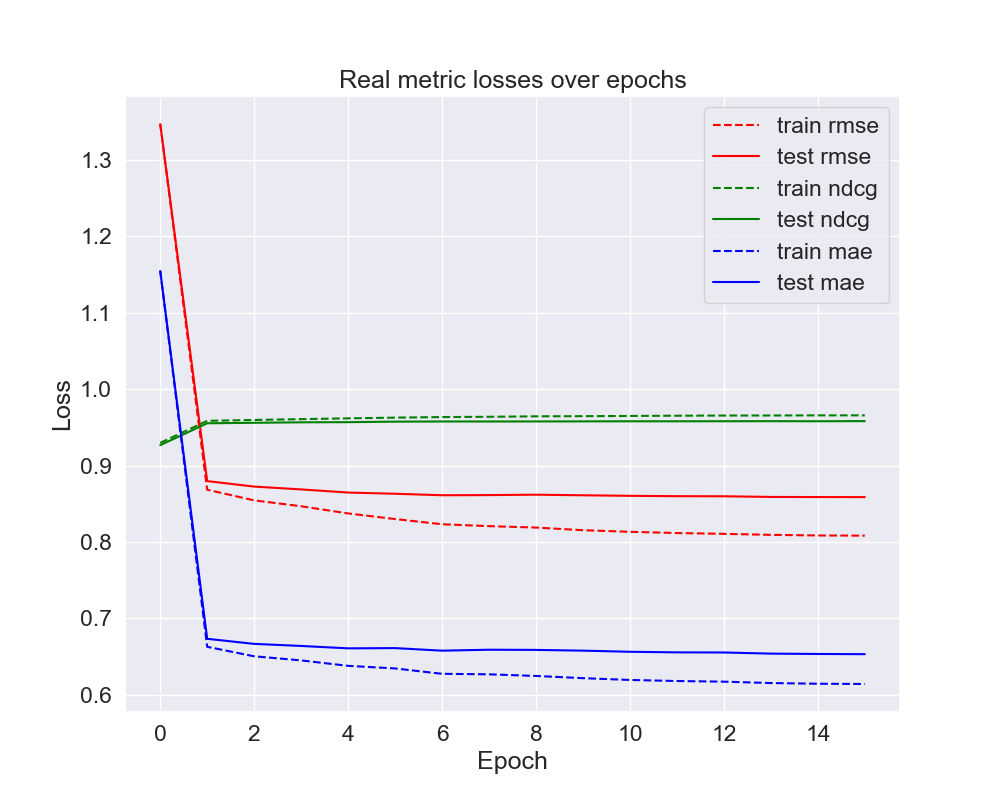
\includegraphics[width=1.0\linewidth]{images/neural_net/real_losses}
\caption{Регрессионные метрики}
\label{fig:nn_real_losses}
\end{minipage}%
\begin{minipage}{.5\textwidth}
\centering
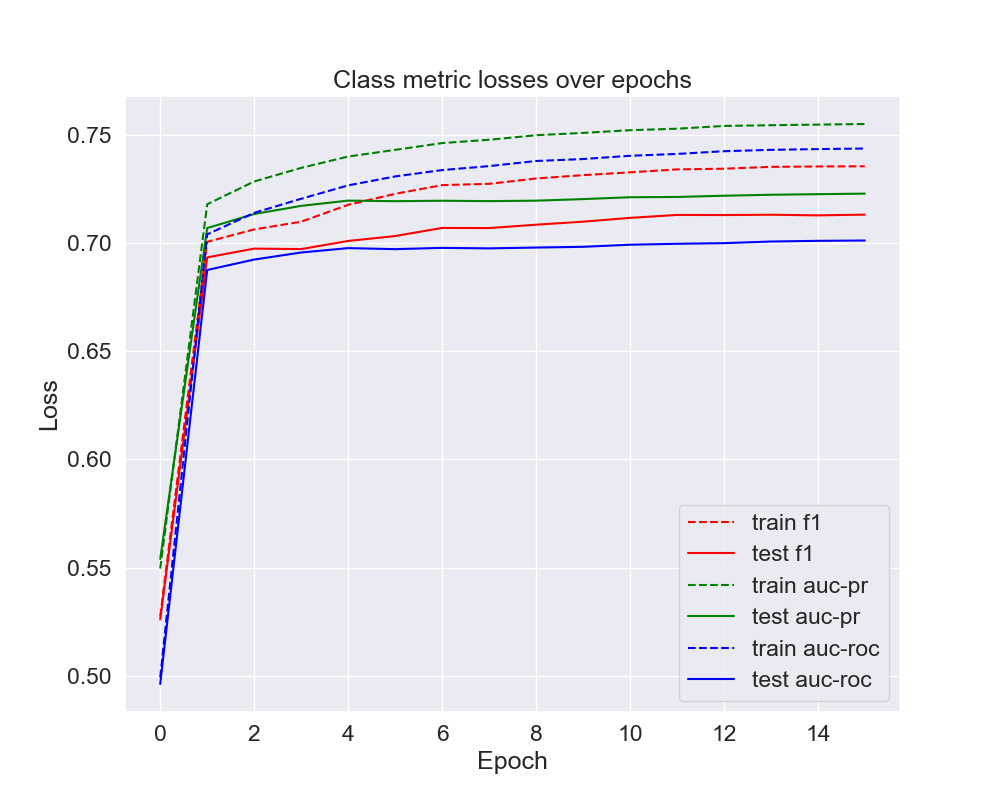
\includegraphics[width=1.0\linewidth]{images/neural_net/class_losses}
\caption{Метрики классификации}
\label{fig:nn_class_losses}
\end{minipage}
\end{figure}

\pagebreak

\subsubsection{Content-based}
Оценка качества представлена в таблице~\ref{tab:content_quality}:

\begin{table}[h]
    \centering{
    \begin{tabular}{ |P{4.8em}|P{4.8em}|P{4.8em}|P{4.8em}|P{4.8em}|P{4.8em}|}
    \hline
    RMSE & MAE & NDCG & F1 & AUC-ROC & AUC-PR \\
    \hline
    1.18735 & 0.8976 & 0.9449 & 0.6693 & 0.6037 & 0.6417 \\
    \hline
    \end{tabular}}
    \caption{Значения метрик}
    \label{tab:content_quality}
\end{table}

Графики ROC/PR-кривых приведены на рисунках~\ref{fig:content_roc},~\ref{fig:content_pr}:

\begin{figure}[h!]
\centering
\begin{minipage}{.5\textwidth}
\centering
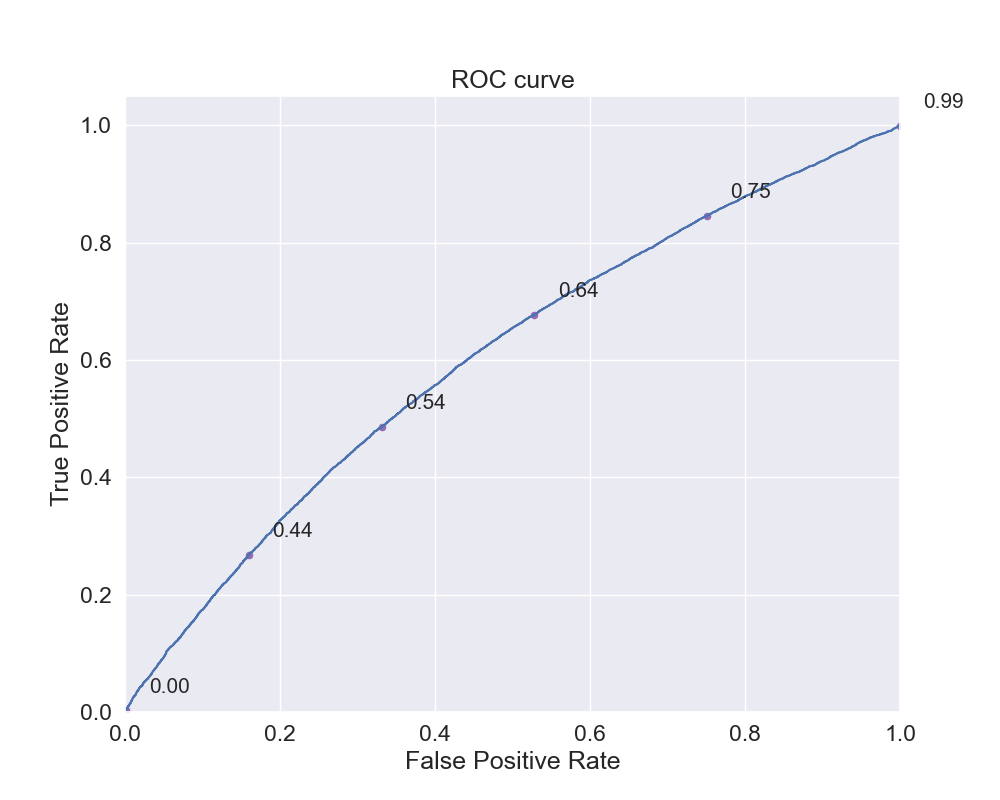
\includegraphics[width=0.9\linewidth]{images/content/roc_curve}
\caption{График ROC-кривой}
\label{fig:content_roc}
\end{minipage}%
\begin{minipage}{.5\textwidth}
\centering
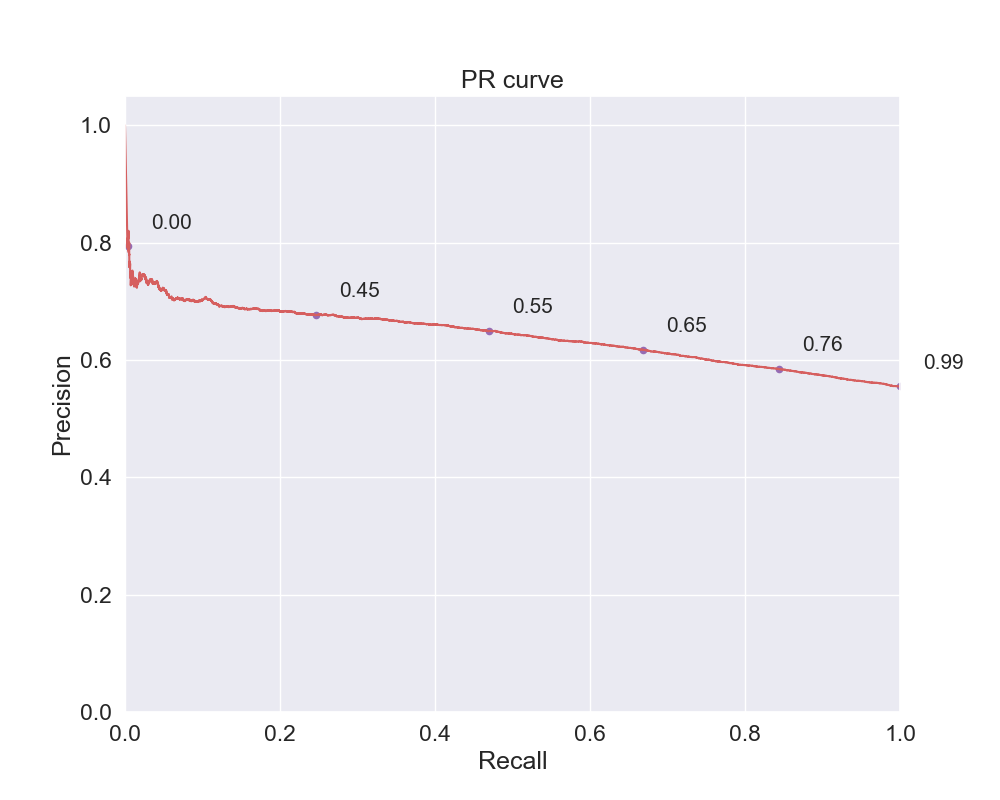
\includegraphics[width=0.9\linewidth]{images/content/pr_curve}
\caption{График PR-кривой}
\label{fig:content_pr}
\end{minipage}
\end{figure}

Среднеквадратическая ошибка автоэнкодера в процессе обучения представлена на рисунке~\ref{fig:autoencoder_losses}:

\begin{figure}[h!]
\centering
\begin{minipage}{0.6\textwidth}
\centering
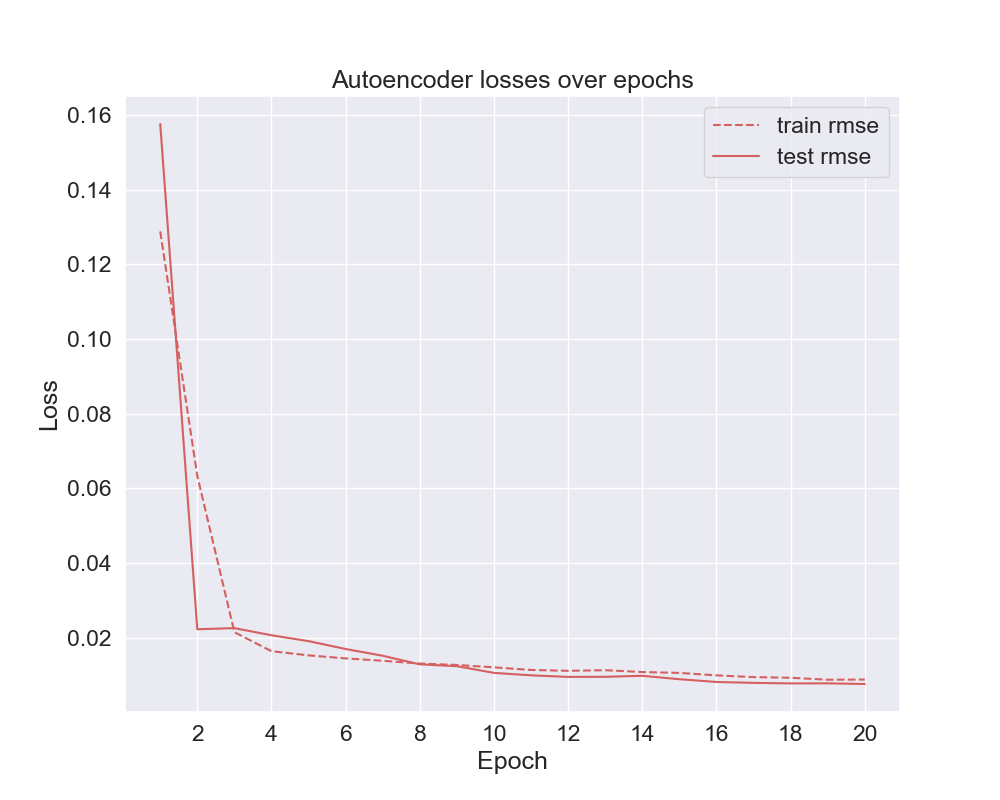
\includegraphics[width=0.85\linewidth]{images/content/autoencoder_losses}
\caption{Среднеквадратическая ошибка автоэнкодера}
\label{fig:autoencoder_losses}
\end{minipage}%
\end{figure}

\pagebreak

\subsubsection{Hybrid}
Для оценки гибридной модели в качестве коллаборативной модели использовалось SGD-разложение, а в качестве контентной - автоэнкодер, обученный сжимать tf-idf пространство тэгов.

Вклад каждой модели варьироваался посредством параметра $\alpha$.
К ответам чистых коллаборативной и контентной моделей относятся значения $\alpha = 0$ и $\alpha = 1$ соответственно:
\begin{equation}\label{eq:hybrid_filtering}
\hat{r}_{ij} = (1 - \alpha)\space SGD(i, j) + \alpha\space C(i, j)
\end{equation}

Оценка качества алгоритма представлена в таблице~\ref{tab:hybrid_quality}:
\vspace{1em}
\begin{table}[h]
    \resizebox{\textwidth}{!}{%
    \begin{tabular}{ |P{4.5em}|P{2.5em}|P{2.5em}|P{2.5em}|P{2.5em}|P{2.5em}|P{2.5em}|P{2.5em}|P{2.5em}|P{2.5em}|P{2.5em}|P{2.5em}|}
    \hline
    $\alpha$ & 0 & 0.1 & 0.2 & 0.3 & 0.4 & 0.5 & 0.6 & 0.7 & 0.8 & 0.9 & 1 \\
    \hline
    RMSE & \cellcolor{green!45}0.8357 & 0.8405 & 0.8535 & 0.8744 & 0.9026 & 0.9374 & 0.9782 & 1.0242 & 1.0748 & 1.1294 & 1.1873 \\
    \hline
    MAE & \cellcolor{green!45}0.6373 & 0.6383 & 0.6461 & 0.6599 & 0.6792 & 0.7040 & 0.7339 & 0.7685 & 0.8077 & 0.8510 & 0.8976 \\
    \hline
    NDCG & 0.9616 & 0.9619 & 0.9623 & \cellcolor{green!45}0.9625 & 0.9620 & 0.9613 & 0.9596 & 0.9581 & 0.9550 & 0.9503 & 0.9449 \\
    \hline
    F1 & 0.7287 & 0.7293 & 0.7312 & \cellcolor{green!45}0.7318 & 0.7315 & 0.7309 & 0.7268 & 0.7199 & 0.7093 & 0.6914 & 0.6693 \\
    \hline
    AUC-ROC & 0.7221 & 0.7233 & 0.7241 & \cellcolor{green!45}0.7242 & 0.7228 & 0.7190 & 0.7116 & 0.6983 & 0.6765 & 0.6443 & 0.6037 \\
    \hline
    AUC-PR & 0.7428 & 0.7439 & 0.7446 & \cellcolor{green!45}0.7446 & 0.7428 & 0.7384 & 0.7309 & 0.7192 & 0.7017 & 0.6754 & 0.6417 \\
    \hline
    \end{tabular}}
    \caption{Значения метрик в зависимости от $\alpha$}
    \label{tab:hybrid_quality}
\end{table}

Графики кривых при $\alpha = 0.3$ представлены на рисунках~\ref{fig:hybrid_roc},~\ref{fig:hybrid_pr}:

\begin{figure}[h!]
\centering
\begin{minipage}{.5\textwidth}
\centering
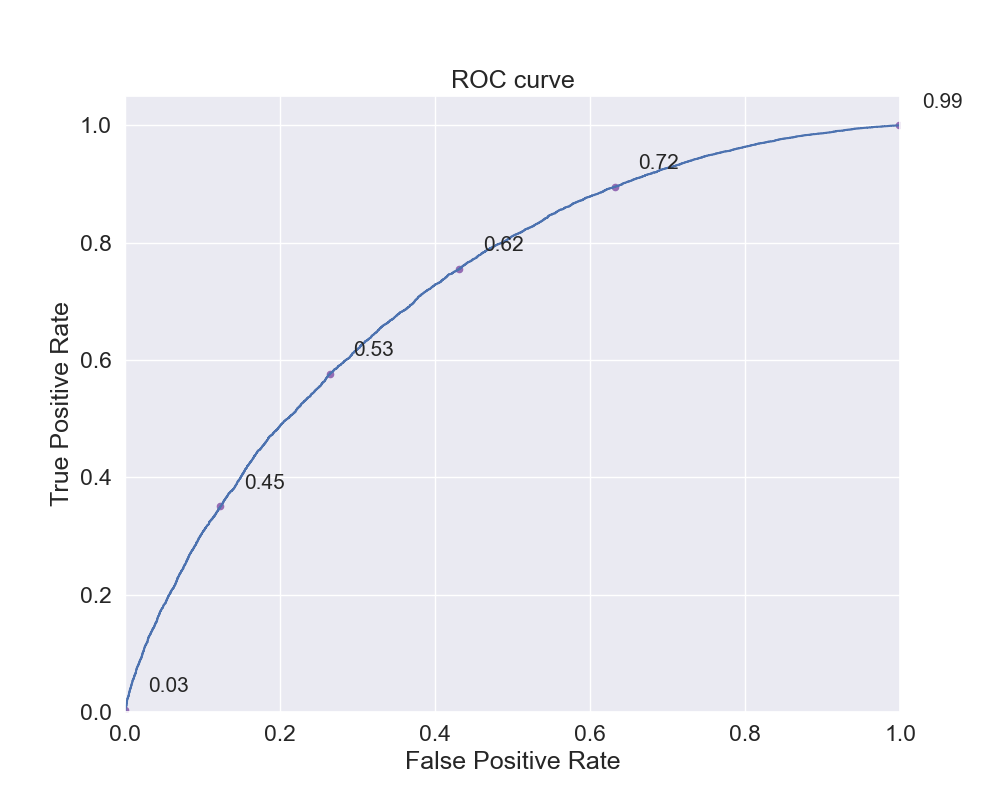
\includegraphics[width=1.1\linewidth]{images/hybrid/roc_curve}
\caption{График ROC-кривой}
\label{fig:hybrid_roc}
\end{minipage}%
\begin{minipage}{.5\textwidth}
\centering
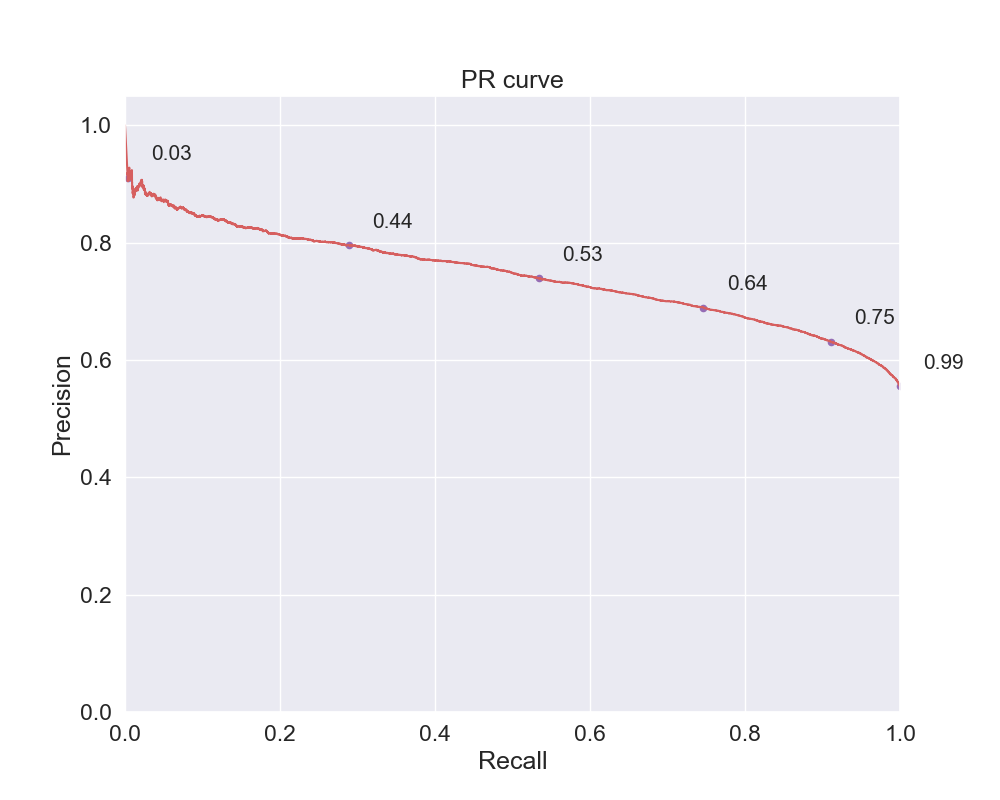
\includegraphics[width=1.1\linewidth]{images/hybrid/pr_curve}
\caption{График PR-кривой}
\label{fig:hybrid_pr}
\end{minipage}
\end{figure}

\pagebreak

\pagebreak

\begin{thebibliography}{1}
\bibitem{resnick} Resnick P., Iacovou N., Suchak M., Bergstrom P., Riedl J. \flqq GroupLens: an open architecture for collaborative filtering of netnews\frqq. Proceedings of the 1994 ACM conference on Computer supported cooperative work, 1994, pp. 175-186.
\bibitem{herlocker} Herlocker J., Konstan J., Borchers A., Riedl J. \flqq An algorithmic framework for performing collaborative filtering\frqq. Proceedings of the 22nd annual international ACM SIGIR conference on Research and development in information retrieval, 1999, pp. 230-237.
\bibitem{breese} Breese J., Heckerman D., Kadie C. \flqq Empirical Analysis of Predictive Algorithms for Collaborative Filtering\frqq.  Proceedings of the Fourteenth conference on Uncertainty in artificial intelligence, 1998, pp. 43-52.
\bibitem{z-score} Herlocker J., Webster J., Jung S., Dragunov A., Holt T., Culter T., Haerer S. \flqq A framework for collaborative information environments and unified access to distributed digital content\frqq. Proceedings of the 2nd ACM/IEEE-CS joint conference on Digital libraries, 2002. pp. 378-378.
\bibitem{chai} Chai T. and Draxler R. \flqq Root mean square error (RMSE) or mean absolute error (MAE)? – Arguments against avoiding RMSE in the literature\frqq. Geosci. Model Dev., 7, 2014, pp. 1247–1250.
\bibitem{l-reg} Andrew Ng \flqq Feature selection, L1 vs. L2 regularization, and rotational invariance\frqq. Proceedings of the twenty-first international conference on Machine learning, 2004, p. 78.
\bibitem{pmf} Mnih A. and Salakhutdinov R. \flqq Probabilistic matrix factorization \frqq. Proceedings of the 20th International Conference on Neural Information Processing Systems, 2007, pp. 1257-1264.
\bibitem{tfidf} Roelleke T. and Wang J. \flqq TF-IDF Uncovered: A Study of Theories and Probabilities \frqq. Proceedings of the 31st Annual International ACM SIGIR Conference on Research and Development in Information Retrieval, 2008, pp. 435-442.
\bibitem{autoencoders} Baldi, Pierre \flqq Autoencoders, Unsupervised Learning and Deep Architectures \frqq. Proceedings of the 2011 International Conference on Unsupervised and Transfer Learning Workshop - Volume 27, 2011, pp. 37-50.
\bibitem{dcg} Järvelin K., Kekäläinen J. \flqq Cumulated gain-based evaluation of IR techniques \frqq. ACM Transactions on Information Systems 20(4), 2002, pp. 422–446.
\bibitem{dcg-log} Wang Y. Wang L., Li Y., Di H., Tie-Yan L., Wei C. \flqq A Theoretical Analysis of NDCG Type Ranking Measures \frqq. Proceedings of the 26th Annual Conference on Learning Theory - Volume 30, 2013.
\end{thebibliography}
\end{document}